%!TEX TS-program = xelatex
%!TEX TS-options = -shell-escape
\newcommand{\verfasser}{Phil Steinhorst}					% Verfasser des Dokuments
\newcommand{\fach}{Elliptische Kurven und Kryptographie}				% Titel der Vorlesung								
\newcommand{\shortFach}{EKK}								% Titel kurz
\newcommand{\prof}{PD Dr. Karin Halupczok}					% Dozent
\newcommand{\untertitel}{gelesen von \prof}					% Untertitel
\newcommand{\semester}{Sommersemester 2015}					% Semester
\newcommand{\homepage}{http://wwwmath.uni-muenster.de/u/karin.halupczok/ellKKSoSe15/}	% Vorlesungshomepage
% % % % % % % % % % % % % % % % % % % % % % % % % % % % % % % % %
%		PhistScript.tex											%
%		XeLaTeX-Konfiguration für Skripte						%
%																%
%		Author: Phil Steinhorst									%
% % % % % % % % % % % % % % % % % % % % % % % % % % % % % % % % %

\RequirePackage[thinlines]{easybmat} %-- muss aufgrund eines Bugs vor etex und tikz geladen werden
\documentclass[a4paper, twoside, headsepline, index=totoc,toc=listof, fontsize=9pt, cleardoublepage=empty, headinclude, DIV=13, BCOR=13mm, titlepage]{scrartcl}

\usepackage{scrtime} 	% KOMA, Uhrzeit ermoeglicht
\usepackage{scrpage2} 	% wie fancyhdr, nur optimiert auf KOMA-Skript, leicht andere Syntax
\usepackage{etoolbox}

\usepackage[usenames, table, x11names]{xcolor}	% Farben. Vor TikZ laden!

% % % TikZ-Pakete % % %
\usepackage{tikz}
\usepackage{tikz-cd}
\usetikzlibrary{external}
\tikzset{>=latex}
\usetikzlibrary{shapes,arrows,intersections}
\usetikzlibrary{calc,3d}
\usetikzlibrary{decorations.pathreplacing,decorations.markings}
\usetikzlibrary{angles}
\tikzexternalize[prefix=tikz/, up to date check=diff]	% -shell-escape-Flag nötig!

% % % verwende LuaLaTeX, wegen dynamischer Speicherallokation
\tikzset{external/system call={xelatex \tikzexternalcheckshellescape 
    -halt-on-error -interaction=batchmode -jobname "\image" "\texsource"}}
    
% % % tikzexternalize für tikzcd deaktivieren, da inkompatibel
\AtBeginEnvironment{tikzcd}{\tikzexternaldisable}
\AtEndEnvironment{tikzcd}{\tikzexternalenable}

% % % um Inkompatibilitaeten von quotes und polyglossia bzw. babel zu vermeiden
\tikzset{
  every picture/.append style={
    execute at begin picture={\shorthandoff{"}},
    execute at end picture={\shorthandon{"}}
  }
}
\usetikzlibrary{quotes}
\usepackage{pgfplots}

% % % Mathe-Zeugs
\usepackage{mathtools} 						% beinhaltet amsmath
\mathtoolsset{showonlyrefs, centercolon}
\usepackage{wasysym}
\usepackage{amssymb} 						% zusätzliche Symbole
\usepackage{latexsym} 						% zusätzliche Symbole
\usepackage{stmaryrd} 						% für Blitz
\usepackage{nicefrac} 						% schräge Brüche
\usepackage{cancel} 						% Befehle zum Durchstreichen
\usepackage{extarrows}						% mehr Pfeile
\usepackage{mathdots}
\DeclareSymbolFont{bbold}{U}{bbold}{m}{n}
\DeclareSymbolFontAlphabet{\mathbbold}{bbold}
\newcommand{\mathds}[1]{\mathbb{#1}} 		% um Kompatibilitaet mit frueheren Benutzung von dsfont herzustellen
\def\mathul#1#2{\color{#1}\underline{{\color{black}#2}}\color{black}} %farbiges Untersteichen im Mathe-Modus

% % % XeTeX & Fonts
\usepackage{mathspec} 						% beinhaltet fontspec 
\usepackage{polyglossia} 					% babel-Ersatz
\setmainlanguage[spelling=new,babelshorthands=false]{german}
\newcommand\glqq{"}
\newcommand\grqq{"}
\defaultfontfeatures{Mapping=tex-text, WordSpace={1.4},Extension=.otf} %
\setmainfont{SourceSansPro}[%
	UprightFont=*-Regular,
	BoldFont=*-Semibold,
	ItalicFont=*-LightIt,
	BoldItalicFont=*-SemiboldIt,
	SmallCapsFont={LinLibertine_R.otf},
	SmallCapsFeatures={Letters=SmallCaps}]
\setsansfont{SourceSansPro}[%
	UprightFont=*-Regular,
	BoldFont=*-Semibold,
	ItalicFont=*-LightIt,
	BoldItalicFont=*-SemiboldIt,
	SmallCapsFont={LinLibertine_R.otf},
	SmallCapsFeatures={Letters=SmallCaps}]
\setmonofont{SourceCodePro}[Scale=0.9,UprightFont=*-Regular, BoldFont=*-Semibold, ItalicFont=*-Light] 
\usepackage{xltxtra}
\usepackage{fontawesome}

% % % Misc.
\usepackage[neverdecrease]{paralist}
\usepackage[german=quotes]{csquotes}
\usepackage{booktabs}
\usepackage{wrapfig}
\usepackage{float}
\usepackage[margin=10pt, font=small, labelfont=sf, format=plain, indention=1em]{caption}
\captionsetup[wrapfigure]{name=Abb. }
\usepackage{stackrel}
\usepackage{ifthen}
\usepackage{multicol}
%\flushbottom

% % % Unterstreichung
\usepackage[normalem]{ulem}
\setlength{\ULdepth}{1.8pt}

% % % Indexverarbeitung
\usepackage{makeidx}
\newcommand{\bet}[1]{\textbf{#1}}
\newcommand{\Index}[1]{\textbf{#1}\index{#1}}
\makeindex
\renewcommand{\indexpagestyle}{scrheadings}

% % % Marginnote & todonotes
\usepackage{marginnote}
\renewcommand*{\marginfont}{\color{gray} \footnotesize }
\usepackage[textsize=small]{todonotes}
\makeatletter
\renewcommand{\todo}[2][]{\tikzexternaldisable\@todo[#1]{#2}\tikzexternalenable}
\makeatother

% % % Konfiguration von Hyperref pdfstartview=FitH, 
\usepackage[hidelinks, pdfpagelabels,  bookmarksopen=true, bookmarksnumbered=true, linkcolor=black, urlcolor=RoyalBlue3, plainpages=false, hypertexnames=false, citecolor=black, hypertexnames=true, pdfauthor={\verfasser}, pdfborderstyle={/S/U}, linkbordercolor=RoyalBlue3, colorlinks=true, unicode, pdfencoding=auto]{hyperref}

\newcommand{\RM}[1]{\MakeUppercase{\romannumeral #1{}}} 	% Römische Zahlen
\usepackage{ellipsis}										% Punkte

% % % % % % % % % % % % % % % % % % % % % % % % % % % % % % % % %
%		PhistMath.tex											%
%		Weitere Mathe-Befehle									%
%																%
%		Author: Phil Steinhorst									%
% % % % % % % % % % % % % % % % % % % % % % % % % % % % % % % % %

% % % Buchstaben und Zahlen
\newcommand{\aff}{\mathbb{A}}
\newcommand{\CC}{\mathbb{C}}
\newcommand{\FF}{\mathbb{F}}
\newcommand{\HH}{\mathbb{H}}
\newcommand{\KK}{\mathbb{K}}
\newcommand{\NN}{\mathbb{N}}
\newcommand{\OO}{\mathbb{O}}
\newcommand{\QQ}{\mathbb{Q}}
\newcommand{\RR}{\mathbb{R}}
\newcommand{\ZZ}{\mathbb{Z}}
\newcommand{\bigO}{\mathcal{O}}					% Landau-O
\newcommand{\ind}{1\hspace{-0,8ex}1} 			% Indikatorfunktion (Doppeleins)

% % % Abk�rzungen
\newcommand{\ab}[1]{\overline{#1}}					% Abschluss
\newcommand{\assoz}{\mathrel{\hat=}}				% assoziiert
\newcommand{\bewrueck}{\glqq$\Leftarrow$\grqq:} 	% Beweis R�ckrichtung
\newcommand{\bewhin}{\glqq$\Rightarrow$\grqq:}		% Beweis Hinrichtung
\newcommand{\borel}{\mathfrak{B}}					% Borelsche Sigma-Algebra
\newcommand{\maxid}{\mathfrak{m}}					% maximales Ideal
\newcommand{\setone}{\{1\}}							% Einsmenge
\newcommand{\leb}{\lambda \hspace{-0,95ex}\lambda}	% Lebesgue-Ma� (Doppel-Lambda)
\newcommand{\Lp}{\mathcal{L}}						% L^p-R�ume
\newcommand{\NT}{\trianglelefteq}					% Normalteiler
\newcommand{\setnull}{\{0\}}						% Nullmenge
\newcommand{\weak}{\rightharpoonup}					% schwache Konvergenz
\newcommand{\weaks}{\overset{*}{\rightharpoonup}}	% schwache *-Konvergenz
\newcommand{\salg}{\mathfrak{A}}					% Sigma-Algebra (Skript-A)
\newcommand{\zyklot}[1]{#1^{(\infty)}}				% zyklotomische Erweiterung


% % % Operatoren
\DeclareMathOperator{\Alt}{Alt} 					% Alternierende n-Linearform
\DeclareMathOperator{\Aut}{Aut} 					% Automorphismen
\DeclareMathOperator{\Bil}{Bil} 					% Bilinearformen
\DeclareMathOperator{\bild}{Bild} 					% Bild
\DeclareMathOperator{\Char}{char} 
\DeclareMathOperator{\dom}{dom} 					% Domain
\DeclareMathOperator{\diam}{diam}					% Durchmesser
\DeclareMathOperator{\dist}{dist} 					% Distanz
\DeclareMathOperator{\eqs}{\mathrel{\widehat{=}}}	% entspricht
\DeclareMathOperator{\diver}{div} 					% Gradient
\DeclareMathOperator{\EPK}{EPK} 					% Einpunktkompaktifizierung
\DeclareMathOperator{\End}{End} 					% Endomorphismen
\DeclareMathOperator{\esssup}{esssup}				% essentielles Supremum
\DeclareMathOperator{\Gal}{Gal}	 					% Galoisgruppe
\DeclareMathOperator{\ggT}{ggT} 					% ggT
\DeclareMathOperator{\GL}{GL}						% allgemeine lineare Gruppe
\DeclareMathOperator{\grad}{grad} 					% Gradient
\DeclareMathOperator{\Grad}{Grad} 					% Grad
\DeclareMathOperator{\Hess}{Hess} 					% Hesse-Matrix
\DeclareMathOperator{\Hom}{Hom} 					% Homomorphismen
\DeclareMathOperator{\id}{id} 						% identische Abbildung
\DeclareMathOperator{\im}{im} 						% image
\DeclareMathOperator{\Jac}{Jac} 					% Jacobson-Radikal
\DeclareMathOperator{\Kern}{Kern}					% Kern
\DeclareMathOperator{\kgV}{kgV} 					% kgV
\DeclareMathOperator{\Koker}{Koker} 				% Kokern
\DeclareMathOperator{\Cov}{Cov} 					% Kovarianz
\DeclareMathOperator{\Mod}{Mod} 					% Moduln
\DeclareMathOperator{\modu}{mod} 					% Modulo
\DeclareMathOperator{\ord}{ord} 					% Ordnung
\DeclareMathOperator{\der}{\partial}				% Partielle Ableitung
\DeclareMathOperator{\pot}{\mathcal{P}}				% Potenzmenge
\DeclareMathOperator{\prlim}{\varprojlim\limits}	% projektiver Limes
\DeclareMathOperator{\Quot}{Quot}					% Quotientenring
\DeclareMathOperator{\Rang}{Rang} 					% Rang
\DeclareMathOperator{\rot}{rot} 					% Rotation
\DeclareMathOperator{\sgn}{sgn} 					% Signum
\DeclareMathOperator{\Spec}{Spec} 					% Spektrum
\DeclareMathOperator{\SL}{SL} 						% Spezielle lineare Gruppe
\DeclareMathOperator{\SO}{SO} 						% Spezielle orthogonale Gruppe
\DeclareMathOperator{\SU}{SU} 						% Spezielle unit�re Gruppe
\DeclareMathOperator{\Spur}{Spur} 					% Spur
\DeclareMathOperator{\supp}{supp} 					% Tr�ger
\DeclareMathOperator{\Sym}{Sym} 					% Symmetrische Gruppe
\DeclareMathOperator{\tr}{tr} 						% trace

% % % Klammerungen
\DeclarePairedDelimiter{\abs}{\lvert}{\rvert}		% Betrag
\DeclarePairedDelimiter{\ceil}{\lceil}{\rceil}		% aufrunden
\DeclarePairedDelimiter{\floor}{\lfloor}{\rfloor}	% aufrunden
\DeclarePairedDelimiter{\sprod}{\langle}{\rangle}	% spitze Klammern
\DeclarePairedDelimiter{\enbrace}{(}{)}				% runde Klammern
\DeclarePairedDelimiter{\benbrace}{\lbrack}{\rbrack}			% eckige Klammern
\DeclarePairedDelimiter{\penbrace}{\{}{\}}			% geschweifte Klammern

% % % Norm
\DeclarePairedDelimiter\doppelstrich{\Vert}{\Vert}
\newcommand{\norm}[2][\relax]{
\ifx#1\relax \ensuremath{\doppelstrich*{#2}}
\else \ensuremath{\doppelstrich*{#2}_{#1}}
\fi}							% selbst definierte Mathe-Befehle

\setlength\parindent{0pt}             % ohne Einrueckung
\renewcommand{\baselinestretch}{1.2}
% % % Konfiguration von scrheadings
\setheadsepline{1pt}[\color{black}]
\pagestyle{scrheadings}
\clearscrheadfoot

% % % Kopf-/Fußzeilenlayout
\providecommand{\shortFach}{\fach}
\ohead{\small \leftmark}
\ofoot[{ \small \thepage}]{ \small \thepage} 
\automark{section}

% Metadaten
\title{\fach}
\author{\verfasser}
\subtitle{\untertitel}
\date{\semester}

% Inhaltsverzeichnis
\usepackage[tocindentauto]{tocstyle}
\usetocstyle{KOMAlike}	

% ntheorem package
\usepackage[hyperref]{ntheorem}			% Lade ntheorem mit hyperref-Workaround
\theoremstyle{break}					% Zeilenumbruch nach Theoremkopf
\theoremheaderfont{\usekomafont{disposition}} % Benutze die gleiche Schriftart, wie für \section \subsection etc.
\theorembodyfont{\normalfont}			% nicht kursiv
\theorempreskipamount0.5cm				% Abstand vor Theorem
\theorempostskipamount0.5cm				% Abstand nach Theorem

% Workaround für Tabulatoren im Theorem-Verzeichnis
\makeatletter
\def\thm@@thmline@name#1#2#3#4{%
        \@dottedtocline{-2}{0em}{2.3em}%
                   {\makebox[\widesttheorem][l]{#1 \protect\numberline{#2}}#3}%
                   {#4}}
\@ifpackageloaded{hyperref}{
\def\thm@@thmline@name#1#2#3#4#5{%
    \ifx\\#5\\%
        \@dottedtocline{-2}{0em}{2.3em}%
            {\makebox[\widesttheorem][l]{#1 \protect\numberline{#2}}#3}%
            {#4}
    \else
        \ifHy@linktocpage\relax\relax
            \@dottedtocline{-2}{0em}{2.3em}%
                {\makebox[\widesttheorem][l]{#1 \protect\numberline{#2}}#3}%
                {\hyper@linkstart{link}{#5}{#4}\hyper@linkend}%
        \else
            \@dottedtocline{-2}{0em}{2.3em}%
                {\hyper@linkstart{link}{#5}%
                  {\makebox[\widesttheorem][l]{#1 \protect\numberline{#2}}#3}\hyper@linkend}%
                    {#4}%
        \fi
    \fi}
}
\makeatother
\newlength\widesttheorem
\AtBeginDocument{
  \settowidth{\widesttheorem}{Proposition 10.10\quad}	% Referenzstring für die Breite der ersten Spalte
}

\newcommand{\qed}{\ifmmode \tag*{$\square$} \else \hfill $\square$ \fi} % qed-Symbol.

							% XeLaTeX-Konfiguration für Skripte
\usepackage{easybmat}
% % % Dokumentspezifische Einstellungen % % %
\setcounter{tocdepth}{3}				% Tiefe im Inhaltsverzeichnis (1: nur Sections, 2: auch subsections...)

\numberwithin{equation}{section}			% Section in Equation-Nummerierung einbeziehen
\newcounter{counter}						% Zähler für Sätze
\newcounter{lecture}
\numberwithin{counter}{lecture}		% Section in Satz-Nummerierung einbeziehen

\newcommand{\nextlecture}{\stepcounter{lecture} \setcounter{counter}{0}}


% ab hier können neue Umgebungen für Sätze definiert und benannt werden!
% Syntax: \newtheorem{interner Umgebungsname}[Zähler]{Name im Dokument}
% Möchte man Sätze und Definitionen getrennt durchnummerieren, benötigt man weitere Zähler.
\theoremlisttype{optname}					% nur Theoreme auflisten, die einen Namen haben. 
\newtheorem{satz}[counter]{Satz}
\newtheorem{defn}[counter]{Definition}
\newtheorem{bem}[counter]{Bemerkung}
\newtheorem{bsp}[counter]{Beispiel}
\newtheorem{lemma}[counter]{Lemma}
\newtheorem{folg}[counter]{Folgerung}
\newtheorem{zusatz}[counter]{Zusatz}
\newtheorem{anw}[counter]{Anwendung}
\newtheorem{erl}[counter]{Erläuterung}
\newtheorem{mot}[counter]{Motivation}
\newtheorem{bew}[counter]{Beweis}
\newtheorem{kor}[counter]{Korollar}
\newtheorem{vor}[counter]{Vorbereitung}
% % % % % % % % % % % % % % % % % % % % % % %
\newcommand{\PP}{\mathbb{P}}
\DeclareMathOperator{\li}{li}
\newcommand{\kon}{\equiv}
\newcommand{\oh}{\mathcal{O}}
\newcommand{\cc}{\mathcal{C}}
\DeclareMathOperator{\Res}{Res}
\DeclareMathOperator{\disc}{disc}
\DeclareMathOperator{\Rg}{Rg}
\newcommand{\pol}{\mathcal{P}}
\newcommand{\leg}[2]{\enbrace*{\frac{#1}{#2}}}

% % % % % % % % % % % % % % % % % % % % % % %
\begin{document}
%!TEX root = ../LA2.tex
\begin{titlepage}
	% Nach einer Vorlage von http://www.LaTeXTemplates.com
	\newcommand{\HRule}{\rule{\linewidth}{0.8mm}} % Defines a new command for the horizontal lines, change thickness here

	\center % Center everything on the page
 
	\begin{minipage}{0.4\textwidth}
	\begin{flushleft}
	
\includegraphics[height=1.5cm,keepaspectratio]{../!config/Bilder/wwulogo.pdf}\\[1cm]
	\end{flushleft}
	\end{minipage}
	\hfill
	\begin{minipage}{0.4\textwidth}
	\begin{flushright}
	\vspace*{0.3cm}
	
\includegraphics[height=1.2cm,keepaspectratio]{../!config/Bilder/fb10logo.pdf} \
	\end{flushright}
	\end{minipage}

	\vspace{2cm}
	


	\HRule \\[0.8cm]
	{ \huge \sffamily\bfseries Lineare Algebra II}\\[0.4cm] % Title of your document
	\HRule \\[1cm]
 
	{\LARGE gelesen von} \\[.7cm]
	\textsc{\LARGE \textbf{Prof. Dr. Siegfried Echterhoff}}\\[.7cm]
	{\LARGE im Sommersemester 2016}\\[2cm]


	\vfill
	{\Large Vorlesungsmitschrift von Phil Steinhorst} \\[.5cm]
	{\large Stand: \today}
	
\end{titlepage}							% Titelseite ausgeben
%!TEX root = ../EKK_SS15.tex
\begin{abstract}
	\section*{Vorwort}
	\label{sec:preface}
	Der vorliegende Text ist eine inhaltliche Aufbereitung zur Vorlesung \textit{Elliptische Kurven und Kryptographie}, gelesen von PD Dr. Karin Halupczok an der WWU Münster im Sommersemester 2015. Der Inhalt entspricht weitestgehend dem handschriftlichen Skript, welches auf der Vorlesungswebsite bereitsgestellt wird. Dieses Werk ist daher keine Eigenleistung des Autors und wird nicht von der Dozentin der Veranstaltung korrekturgelesen. Für die Korrektheit des Inhalts wird keinerlei Garantie übernommen. Bemerkungen, Korrekturen und Ergänzungen kann man folgenderweise loswerden:
	\begin{itemize}
		\item persönlich durch Überreichen von Notizen oder per E-Mail
		\item durch Abändern der entsprechenden \TeX-Dateien und Versand per E-Mail an mich
		\item direktes Mitarbeiten via GitLab. Dieses Skript befindet sich im \texttt{LaTeX-WWU}-Repository von Jannes Bantje:
		\begin{center}
			\url{https://gitlab.com/JaMeZ-B/latex-wwu}
		\end{center}
	\end{itemize}
	
	\subsection*{Literatur}
	\label{sub:lit}
	\begin{itemize}
		\item Blake, Seroussi, Smart: Elliptic curves in cryptography \cite{BlakeSeroussiSmart}
		\item Menezes, van Oorschot, Vanstone: Handbook of applied cryptography \cite{MenezesOorschotVanstone}
		\item Silverman: The arithmetic of elliptic curves \cite{SilvermanEC}
		\item Silverman: A friendly introduction to number theory, chap. 40-45 \cite{SilvermanNT}
		\item Washington: Elliptic curves, number theory and cryptography \cite{Washington}
		\item Werner: Elliptische Kurven in der Kryptographie \cite{Werner}
	\end{itemize}
	
	\subsection*{Kommentar der Dozentin}
	In der Vorlesung beschäftigen wir uns mit den arithmetischen und geometrischen Eigenschaften elliptischer Kurven sowie deren Anwendungen in der Kryptographie. Dabei werden wir auch einen Vergleich mit Anwendungen der elementaren Zahlentheorie in der Kryptographie ziehen. Wir verfolgen eine elementare Herangehensweise, d.h. Kenntnisse der algebraischen Geometrie und der Funktionen- oder Zahlentheorie werden nicht benötigt. Es genügen die Vorkenntnisse aus den Grundvorlesungen.
	\newpage	
	\subsection*{Vorlesungswebsite}
	\label{sub:link}
	Das handgeschriebene Skript sowie weiteres Material findet man unter folgendem Link:
	\begin{center}
		\url{http://wwwmath.uni-muenster.de/u/karin.halupczok/ellKKSoSe15/}
	\end{center}
	
	\vfill
	\begin{flushright}
		Phil Steinhorst \\
		p.st@wwu.de
	\end{flushright}
	\newpage
\end{abstract}
\cleardoubleemptypage
\tableofcontents
\newpage											% Inhaltsverzeichnis ausgeben
\setcounter{section}{-1}
\section{Motivation und Einführung}
\label{sec:para0}

\nextlecture
\subsection*{Kryptologie}
	Die \textbf{Kryptologie} besteht aus den folgenden beiden Gebieten: \marginnote{[1]} 
	\begin{description}
		\item[Kryptographie:] Studium mathematischer Techniken zur Verschlüsselung von Informationen oder geheimen Nachrichten und dem Schutz von Daten.
		\item[Kryptoanalyse:] Beschreibung der Rückgewinnung von Informationen aus verschlüsselten Texten, der Entschlüsselung.
	\end{description}
Oft meint man mit "Kryptographie" die Kryptologie. \\

Früher wurde die Kryptographie vor allem im militärischen oder diplomatischen Sektor verwendet, heutzutage steht in unserer vernetzten Welt vor allem auch der praktische Nutzen im Alltag im Vordergrund: im Internet einkaufen, Online-Banking, persönliche Daten geheimhalten bzw. Datenschutz, Nachrichten und Dokumente digital unterschreiben etc. 
Das Internet liefert schnelle Informationswege über öffentliche Kanäle, die leicht abgehört werden können, sodass die Verschlüsselung schützenswerter Daten unumgänglich wird. 
Auch die Möglichkeit zur Signierung wird nötig, weil sehr leicht Absenderangaben gefälscht werden können. 
Eventuell nicht abhörsichere Kanäle können außer dem Internet aber auch Briefe, Radio, Boten, etc. sein. \\

Bei der \textbf{symmetrischen Verschlüsselung} von Daten gibt es einen Sender $S$ und einen Empfänger $E$, die sich beide auf einen gemeinsamen Schlüssel geeinigt haben, der zum Ver- und Entschlüsseln dient. 
Beim \Index{Caesar-Code} z.B. ist dies die Vereinbarung, jeden Buchstaben durch den dritten nachfolgenden im Alphabet zu ersetzen, also $A \mapsto D, B \mapsto E, C \mapsto F$, usw. 
Die Entschlüsselung ist klar. 
Derartige \textbf{monoalphabetische Chiffrierungen}, bei der jeder Buchstabe des Alphabets stets durch denselben Geheimtextbuchstaben chiffriert wird, sind durch Häufigkeitsanalysen durch einen Angreifer, der die verschlüsselten Nachrichten abhört, sehr leicht zu entschlüsseln. 
Übrigens gibt es auch heutzutage PDF-Verschlüsselungsprogramme, die so arbeiten! 

In dieser Vorlesung behandeln wir die heutzutage gängigen modernen Methoden, die als sicher gelten. 
Worauf diese starke Sicherheit beruht, hat mathematische Gründe, die wir besprechen möchten. 
Vor allem interessiert uns, wie und welche Mathematik in die Kryptologie kommt, sodass wir deren Verfahren verstehen können. \\

Die Anwendungen erfordern die Lösung folgender Probleme bei symmetrischen Verschlüsselungsverfahren:
\begin{itemize}
	\item Schlüsselaustausch über öffentliche Kanäle (\textbf{öffentliche Schlüssel})
	\item Verschlüsselung ohne vorherigen Schlüsselaustausch (mit \textbf{geheimen Schlüsseln}, die nicht versendet werden)
	\item Digitale Signierung und Autentifizierung
\end{itemize}
Dies können \textbf{asymmetrische Verfahren} leisten (auch \textbf{Public Key-Kryptographie} genannt) und gehen zurück auf Ideen von Diffie\footnote{Whitfield Diffie, \url{http://de.wikipedia.org/wiki/Whitfield_Diffie}} und Hellman\footnote{Martin Hellman, \url{http://de.wikipedia.org/wiki/Martin_Hellman}} aus den 70er Jahren: \\

Jeder Nutzer eines Kommunikationskanals hat einen privaten Schlüssel, den er geheim hält und niemand sonst kennt, sowie einen öffentlichen Schlüssel, den jeder einsehen kann. 
Eine Nachricht wird dann unter Ausnutzung einer Funktion $x \mapsto f(x)$ verschlüsselt, die zwar leicht zu berechnen, aber praktisch nur mit Kenntnis des privaten Schlüssels des rechtmäßigen Empfängers entschlüsselt werden kann. 
Der Sender der Nachricht wird dafür den öffentlichen Schlüssel des Empfängers zur Verschlüsselung benutzen. 
Eine derartige Funktion heißt \Index{Einwegfunktion}.

\minisec{Beispiele}
\begin{itemize}
	\item \Index{RSA-Verfahren}: $(p,q) \mapsto p \cdot q$ mit $p,q$ prim.
	\item \Index{ECC-Verfahren}: $x \mapsto mx$ in einer Gruppe auf einer elliptischen Kurve.
\end{itemize}

In einem ersten Teil der Vorlesung stellen wir gängige Verfahren dar, die leicht mit dem Zahlring $\ZZ$ und Strukturen darin realisiert werden können. 
Dabei werden wir nur einige Hilfsmittel der elementaren Zahlentheorie entwickeln und dafür heranziehen. 
In einem zweiten Teil studieren wir die Eigenschaften elliptischer Kurven als interessante geometrische und arithmetische Objekte, die sich in der Praxis der Kryptographie als nützlich erwiesen haben. 
Wir besprechen dann auch die Sicherheit und Implementierung dieser Verfahren und vergleichen sie miteinander.

\subsection*{Elliptische Kurven}
Was sind elliptische Kurven? Jedenfalls sind elliptische Kurven \textbf{keine} Ellipsen. 
Ellipsen lassen sich durch Gleichungen der Form
\[ \enbrace*{\frac{x}{a}}^2 + \enbrace*{\frac{y}{b}}^2 = 1 \text{ mit } a,b \in \RR \setminus \setnull \]
beschreiben. 
Durch die Parametrisierung $x(t) = a \cdot \cos(t), y(t) = b \cdot \sin(t)$ ergibt sich für die Bogenlänge der Ellipse ein elliptisches Integral zweiter Art, nämlich
\[ \int_{0}^{2\pi} \sqrt{ \enbrace*{\frac{dx(t)}{dt}}^2 + \enbrace*{\frac{dy(t)}{dt}}^2 } dt = 4 \int_{0}^{2\pi} \sqrt{ a^2 \cos^2(t) + b^2 \cdot \sin^2 (t)} dt \]
Im Allgemeinen lässt sich dies nicht elementar integrieren (außer natürlich, falls $a = b$, d.h. ein Kreis vorliegt). 
Mit Hilfe von elliptischen Kurven findet man jedoch nicht-elementare Stammfunktionen für diese Integrale\linebreak ($\Rightarrow$ Funktionentheorie). 
Aufgrund dieses Zusammenhangs haben elliptische Kurven ihren Namen, sie haben ansonsten nichts mit Ellipsen zutun. \\

Was sind nun elliptische Kurven? Es sind "abelsche Varietäten der Dimension 1". 
Elliptische Kurven sind spezielle algebraische Kurven über einem Körper $k$. 
Es handelt sich dabei um glatte kubische Kurven, deren definierende algebraische Gleichung sich meist in die Form
\[ E \colon y^2 = x^3 + ax + b \text{ mit } a,b \in k \]
bringen lässt. 
Als Punktmenge haben wir dafür
\[ E(k) := \{ (x,y) \in k^2 : y^2 = x^3 + ax + b\} \cup \{ \oh \}, \]
die Kurve hängt nur von $a,b$ ab. 
Die Rolle des zusätzlichen so genannten "unendlich fernen Punkts" $\oh$ werden wir dabei noch näher beleuchten. \\

Zwei typische Beispiele für elliptische Kurven:
\begin{enumerate}[1)]
	\item $E_1\colon y^2 = x^3 + 17$, hier liegen sogar Punkte mit ganzzahligen Koordinaten auf $E_1$, nämlich $(-2,3), (-1,4), (2,5)$. 
	Die Kurve besteht aus einer Zusammenhangskomponente.
	\item $E_2 \colon y^2 = x^3 + ax + b$, wenn $f(x) = x^3 + ax + b$ drei verschiedene Nullstellen hat, z.B. $a = -3, b= -1$. 
	Die Kurve besteht dann aus zwei Zusammenhangskomponenten.
\end{enumerate}

\begin{figure}[h!]
	\centering
	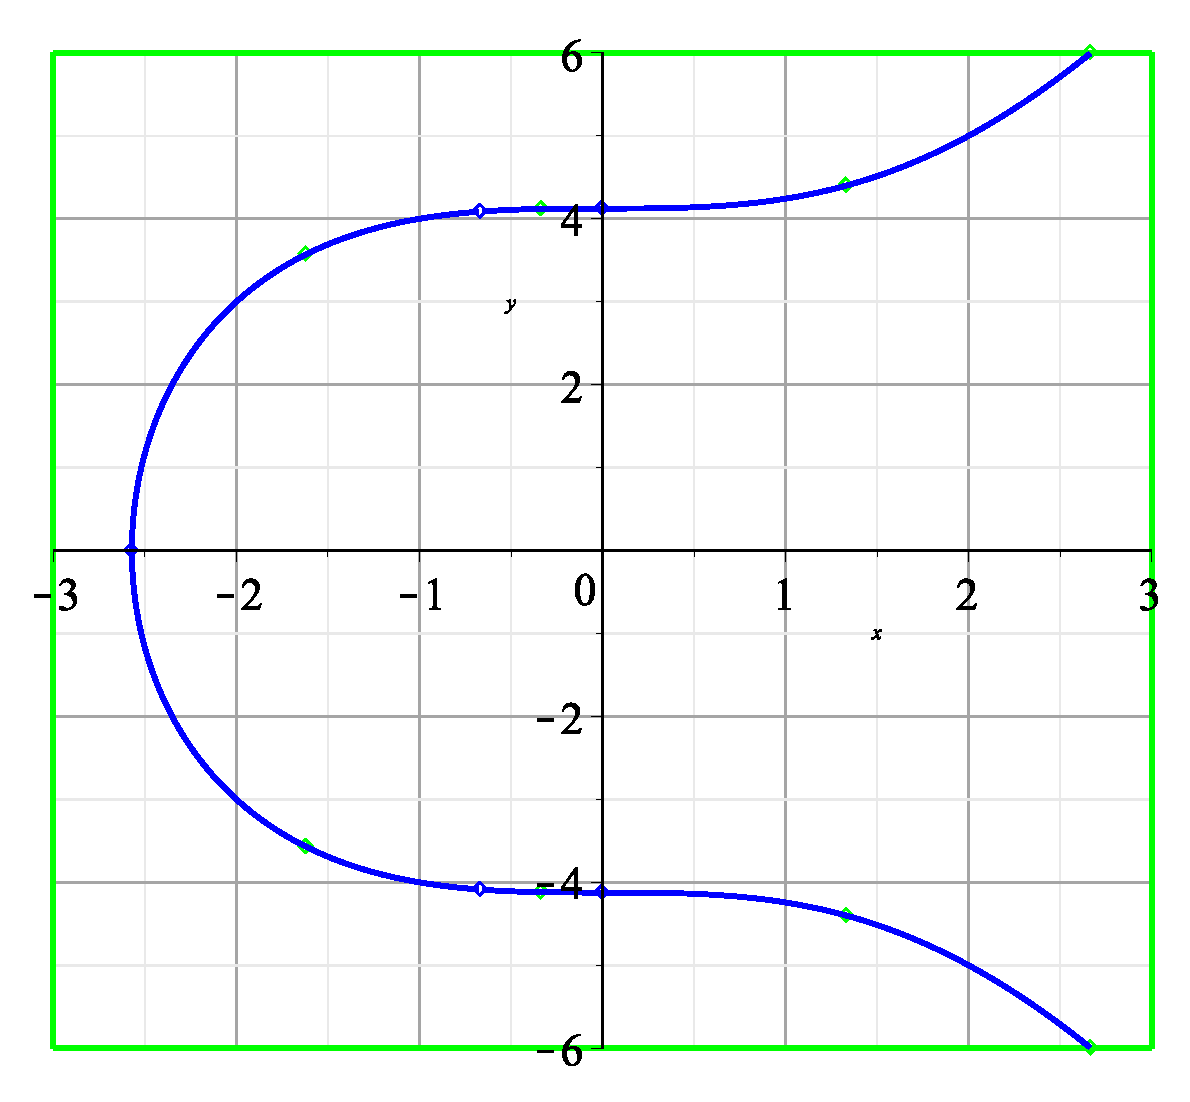
\includegraphics[scale=.3]{img/curve_0_1.eps} \hspace{2cm}
	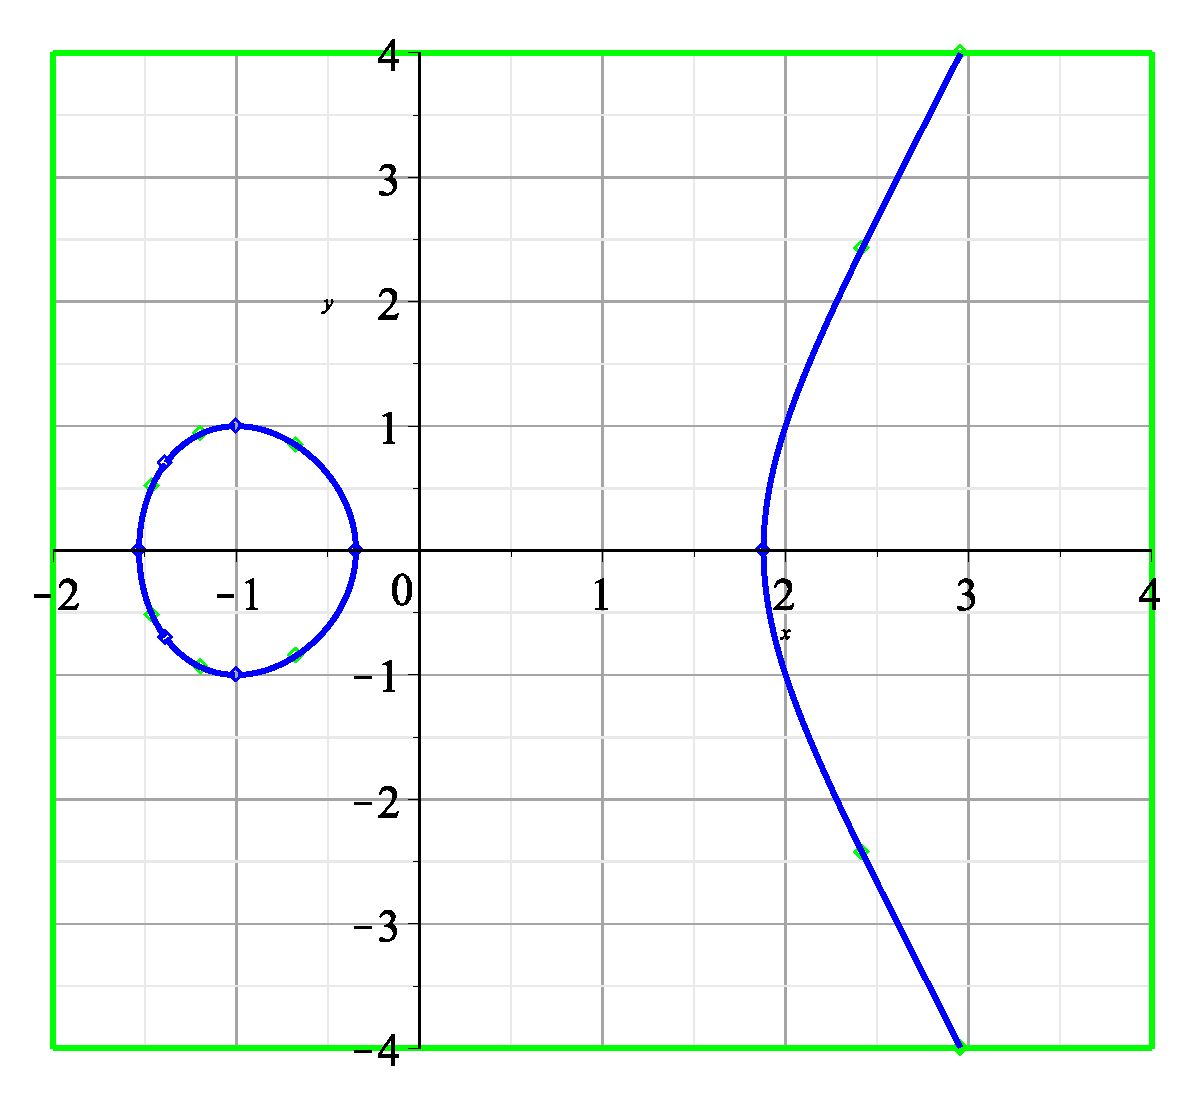
\includegraphics[scale=.3]{img/curve_0_2.eps}
	\caption{Die Kurven $E_1$ (links) und $E_2$ (rechts).}
\end{figure}
%\begin{figure}[h]
%	\centering
%	\begin{tikzpicture}
%	\begin{axis}[
%		scale only axis,
%		xlabel=$x$,
%		ylabel=$y$,
%		grid=major,
%		axis lines=middle,
%		inner axis line style={=>},
%		ymin = -5,
%		ymax = 5,
%		xmin = -3,
%		xmax = 3,
%		xtick={-3,-2,...,3},
%		ytick={-5,-4,...,5}
%	]
%	\addplot[color=red, thick, domain=-2.57128:3, samples=100] {(x^3+17)^(1/2)};
%	\addplot[color=red, thick, domain=-2.57128:3, samples=100] {-(x^3+17)^(1/2)};
%	\end{axis}
%	\end{tikzpicture} \hspace{2cm}
%	\begin{tikzpicture}
%	\begin{axis}[
%		scale only axis,
%		xlabel=$x$,
%		ylabel=$y$,
%		grid=major,
%		axis lines=middle,
%		inner axis line style={=>},
%		ymin = -5,
%		ymax = 5,
%		xmin = -3,
%		xmax = 3,
%		xtick={-3,-2,...,3},
%		ytick={-5,-4,...,5}
%	]
%	\addplot[color=red, thick, domain=-1.53208888:-0.347296, samples=100,unbounded coords=jump] {(x^3-3*x-1)^(1/2)};
%	\end{axis}
%	\end{tikzpicture}
%\end{figure}

\minisec{Bemerkung}
	Die kubischen Kurven $C_1\colon y^2 = x^3 - 3x +2$ und $C_2\colon y^2 = x^3$ z. B. sind jedoch keine elliptischen Kurven, weil diese nicht glatt sind. \\

\begin{figure}[H]
	\centering
	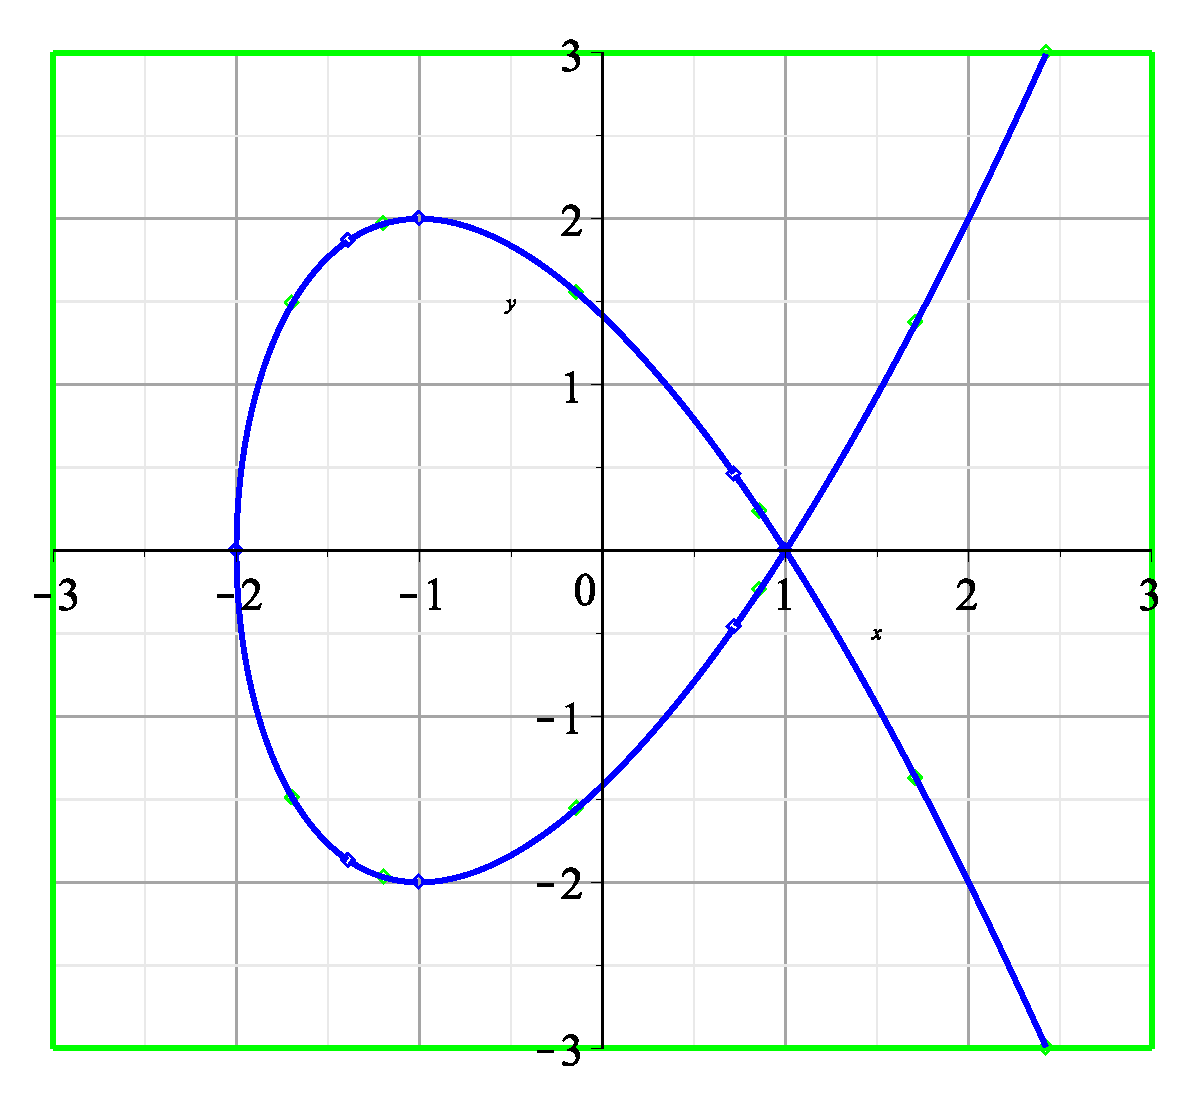
\includegraphics[scale=.3]{img/curve_0_3.eps} \hspace{2cm}
	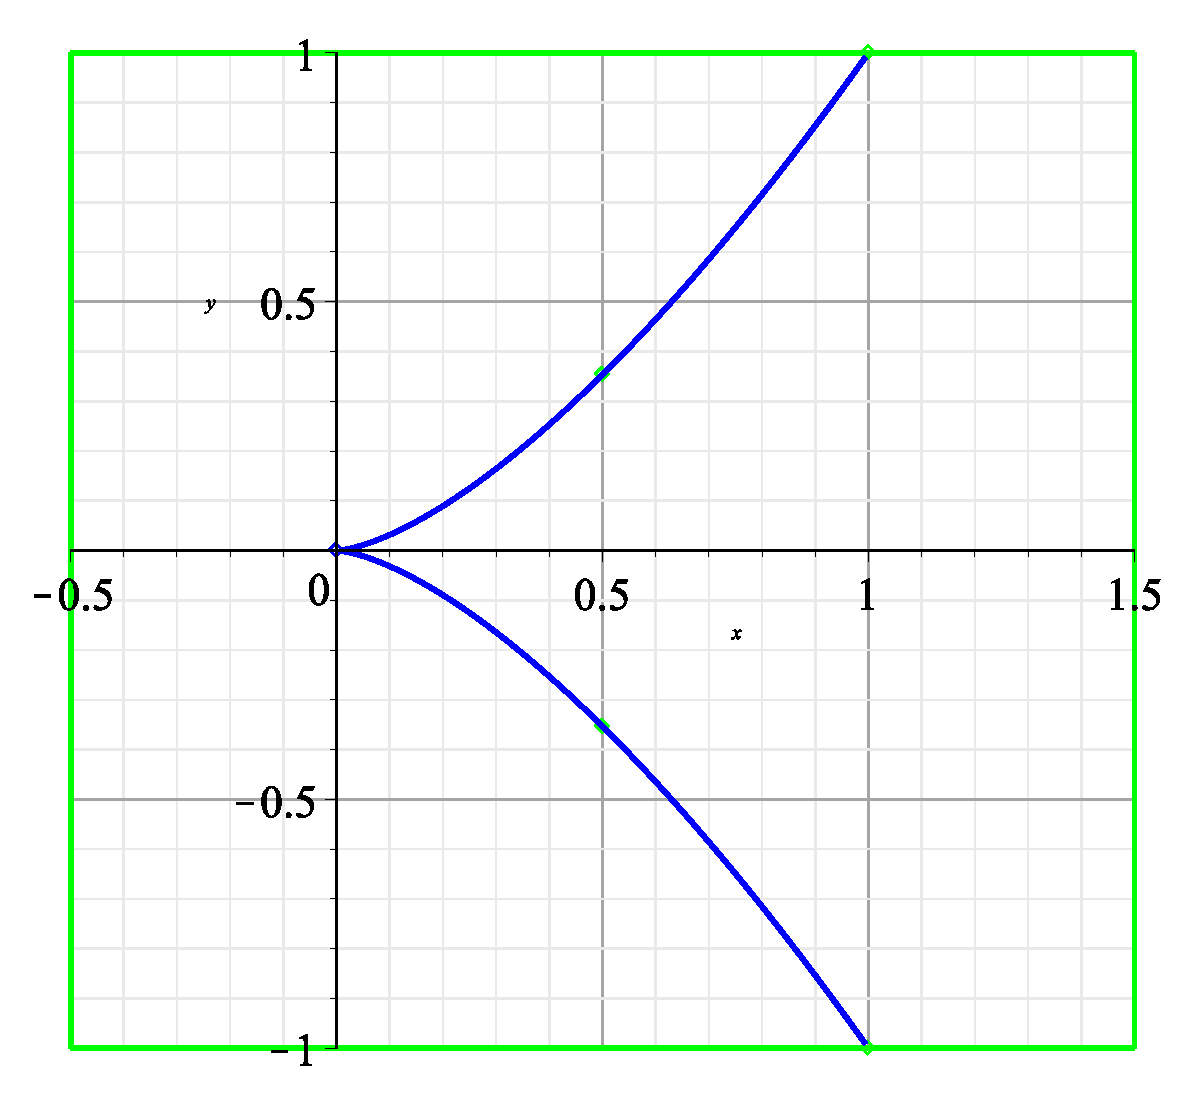
\includegraphics[scale=.3]{img/curve_0_4.eps}
	\caption{Die Kurven $C_1$ (links) und $C_2$ (rechts). $C_1$ ist nicht glatt im Punkt $(1,1)$, $C_2$ nicht im Punkt $(0,0)$.}
	\label{fig:bsp}
\end{figure}

Für die Kryptographie sind elliptische Kurven interessant, weil sich eine Verknüpfung auf ihrer Punktemenge definieren lässt, mit der diese zu einer Gruppe wird. 
Dabei gerade auch endliche Körper $k$ zuzulassen, macht diese Verknüpfung auf Rechenmaschinen realisierbar. 
Die Sicherheit der darauf beruhenden elliptic curve cryptography (ECC) beruht darauf, dass das Problem des diskreten Logarithmus auf einer elliptischen Kurve $E$, nämlich die Umkehrung der Funktion $P \mapsto mP$ für $m \in \NN$ fest, nach heutigem Wissensstand rechnerisch im Allgemeinen extrem schwer realisierbar ist.
\newpage
\section{Fundamentalsatz der elementaren Arithmetik}
\label{sec:para1}

\minisec{Terminologie}
	Sei $R$ ein kommutativer Ring mit $1 \neq 0$. $R$ heißt \Index{Integritätsring} bzw. \bet{nullteilerfrei}, wenn gilt: \index{Nullteiler} \marginnote{14.10.\\ \ [1]}
	\[ a \cdot b = 0 \quad \Rightarrow \quad a = 0 \text{ oder } b = 0.\]

\begin{bsp} \label{bsp_integritaetsringe}
	\begin{itemize}
		\item $\ZZ$
		\item $\ZZ[\sqrt{2}] := \{a + b\sqrt{2} : a,b \in \ZZ \} \subseteq \RR$ \\
			$\ZZ[i] := \{a + bi : a,b \in \ZZ\} \subseteq \CC$ \\
			$\ZZ[\sqrt{-5}] := \dots$
		\item $K[X]$ für $K$ Körper \\
			$\ZZ[X]$
		\item $K$ Körper
		\item $\CC \sprod{z} := \penbrace*{\text{konvergente Potenzreihen } \sum\limits_{n=0}^{\infty} a_n z^n}$
		\item Nicht nullteilerfrei ist z.B. $\mathcal{C}[0,1] := \{f \colon [0,1] \rightarrow \RR \text{ stetig} \}$
	\end{itemize}
\end{bsp}

\begin{defn}[Teilbarkeit] \label{def_1.1}
	Seien $a,b \in R$. $a$ heißt ein \Index{Teiler} von $b$, wenn ein $q \in R$ existiert mit $b = qa$. Wir schreiben dann:
	\[ a | b \]
	Ist $R$ nullteilerfrei und $a \neq 0$, so ist $q$ eindeutig bestimmt.
\end{defn}

\begin{falko}[Triviale Teilbarkeitsregeln] \label{F1.1}
	\begin{enumerate}[(i)]
		\item $a | 0, 1 | a, a | a$
		\item $a | b, b | c \quad \Rightarrow \quad a | c$
		\item $a | b, a | c \quad \Rightarrow \quad a | b+c, a | b-c$
		\item $a_1 | b_1, a_2 | b_2 \quad \Rightarrow \quad a_1 a_2 | b_1 b_2$
		\item $ac | bc \quad \Rightarrow \quad a | b$, falls $c \neq 0$ und $R$ nullteilerfrei.
	\end{enumerate}	
\end{falko}

\begin{defn}[Einheit, assoziiert] \label{def_1.2}
	\begin{enumerate}[(i)]
		\item $e \in R$ heißt eine \Index{Einheit} in $R$, falls $e | 1$ gilt, d.h. falls ein $f \in R$ existiert mit $ef = 1$. $f$ ist eindeutig bestimmt. Wir setzen $e^{-1} := f$ und schreiben auch $\frac{1}{e}$ für $e^{-1}$. \\
		Wir bezeichnen die \Index{Einheitengruppe} von $R$ mit $R^\times := \{x \in R : x \text{ ist Einheit in } R\}$.
		\item $a \in R$ heißt \Index{assoziiert} zu $b \in R$, falls $a | b$ und $b | a$ gilt. Schreibe: $a \assoz b$.
	\end{enumerate}
\end{defn}

\newpage
\begin{bsp}
	\begin{enumerate}[1)]
		\item Sei $K$ ein Körper, dann ist $K^\times = K \setminus \setnull$. \qquad $\ZZ^\times = \{1,-1\}$, \qquad $K[X]^\times = K^\times$, \\
		$\mathcal{C}[0,1]^\times = \{f \in \mathcal{C}[0,1] : f(x) \neq 0 \text{ für alle } x \in [0,1]\}$, \qquad  $\ZZ[\sqrt{2}]^\times = \{\pm (1+\sqrt{2})^k : k \in \ZZ \}$ \\
		$\ZZ[X]^\times = \{1, -1\}$ \qquad $\CC \sprod{z}^\times = \penbrace*{ \sum a_n z^n \in \CC \sprod{z} : a_0 \neq 0}$
		\item $e \in R^\times \quad \Leftrightarrow \quad e | a$ für jedes $a \in R$.
	\end{enumerate}
\end{bsp}

\begin{falko} \label{F1.2}
	Sei $R$ ein Integritätsring, $a, b \in R$ und $b \neq 0$. Dann gilt:
	\[ a \assoz b \quad \Leftrightarrow \quad \exists e \in R^\times \text{ mit } b = ea \]
\end{falko}

\minisec{Beweis}
	\begin{description}
		\item[\bewrueck] $a | b, e^{-1}b = a, b | a$
		\item[\bewhin] Da $a | b$ und $b | a$, existieren $e, f \in R$, sodass $b = ea$ und $a = fb$. $\Rightarrow b = efb \Rightarrow ef = 1$, da $b \neq 0$ und $R$ nullteilerfrei. \qed
	\end{description}

\setlength{\fboxsep}{10pt}
\setlength{\fboxrule}{3pt}
\begin{center}
	\fbox{\textbf{Ab jetzt ist, wenn nichts anderes gesagt, $R$ ein Integritätsring!}}
\end{center}

\begin{defn}[unzerlegbar, irreduzibel, zusammengesetzt] \label{def_1.3}
	Sei $a \in R \setminus R^\times$. $a$ heißt \Index{unzerlegbar} oder \Index{irreduzibel} in $R$, wenn gilt:
	\[ a = bc \text{ in } R \quad \Rightarrow \quad b \in R^\times \text{ oder } c \in R^\times. \]
	Andernfalls heißt $a$ \bet{zerlegbar}, \bet{zusammengesetzt} oder \bet{reduzibel}.
\end{defn}

\minisec{Bemerkung}
	$a$ unzerlegbar $\quad \Leftrightarrow \quad $ jeder Teiler von $a$ ist Einheit oder assoziiert zu $a$ \\
	$a$ zerlegbar $\quad \Leftrightarrow \quad a$ hat echten Teiler, d.h. einen Teiler, der weder eine Einheit ist noch assoziiert zu $a$

\setcounter{countdef}{2}
\begin{defn}[Primzahl] \label{def_1.3'}
	Ein $p \in \ZZ$ heißt \Index{Primzahl}, wenn $p \in \NN$ und $p$ unzerlegbar in $\ZZ$. Wir bezeichnen mit $\PP$ die Menge der Primzahlen von $\ZZ$. $a$ unzerlegbar in $\ZZ \Leftrightarrow a = p$ oder $a = -p$ mit $p \in \PP$.
\end{defn}

\minisec{Bemerkung}
	$a \in \ZZ$ sei zerlegbar, $a \neq 0$. Dann gibt es eine Primzahl $p$ mit $p | a$ und $p \leq \sqrt{|a|}$.

\begin{defn}[Zerlegung in unzerlegbare Faktoren] \label{def_1.4}
	Wir sagen, $a \in R$ besitzt in $R$ eine \Index{Zerlegung in unzerlegbare Faktoren}, wenn
	\begin{equation}
	\begin{aligned}
		a = ep_1p_2\dots p_r \text{ mit } e \in R^\times \text{ und } p_1,\dots,p_r \text{ unzerlegbar} \label{eq_def_1.4}
	\end{aligned}
	\end{equation}
	\eqref{eq_def_1.4} heißt eine Zerlegung von $a$ in unzerlegbare Faktoren. Auch $r = 0$ ist erlaubt.
\end{defn}

\begin{falko} \label{F1.3}
	In $\ZZ$ besitzt jedes $a \neq 0$ eine Zerlegung in unzerlegbare Faktoren.
\end{falko}	

\setcounter{countfalko}{2}
\begin{falko} \label{F1.3'}
	Jede natürliche Zahl $a > 1$ besitzt eine Zerlegung $a = p_1p_2 \dots p_r$ mit Primzahlen $p_1,\dots,p_r$ und $r \geq 1$.
\end{falko}

\minisec{Bemerkung}
	\begin{enumerate}[1)]
		\item Die Aussage F1.3 gilt auch für die Beispiele \ref{bsp_integritaetsringe}, mit Ausnahme von $\mathcal{C}[0,1]$.
		\item Sei $R$ ein Integritätsring, der die \Index{Teilbarkeitsbedingung für Hauptideale} erfüllt, so besitzt jedes $a \neq 0$ aus $R$ eine Zerlegung in unzerlegbare Faktoren.
		\item Primzahlen sind die multiplikativen Bausteine (Atome) von $\NN$.
		\item Im Beispiel $\CC\sprod{z}$ von oben gibt es (bis auf Assoziiertheit) nur das einzige unzerlegbare Element $z$. Dieses ist ein \Index{Primelement} (der Begriff folgt weiter unten).
	\end{enumerate}
	
\begin{satz}[Existenz unendlich vieler Primzahlen] \label{satz_1.1}
	Es gibt unendlich viele Primzahlen.
\end{satz}

\textbf{Bemerkungen} \\
	Es sei $p_1,p_2,\dots$ die aufsteigend sortierte Folge der Primzahlen.
	\begin{enumerate}[1)]
		\item $a_n := p_1p_2\dots p_n +1$ ist Primzahl für $n \leq 5$, aber z.B. nicht für $n = 6$. Unklar ist, ob unendlich viele $a_n$ Primzahlen oder keine Primzahlen sind.
		\item Für $x \in \RR_{>0}$ definieren wir:
		\[ \pi(x) := \# \penbrace{p \in \PP : p \leq x}\]
	\end{enumerate}

\minisec{Primzahlsatz (Gauß, Legendre)}
	\begin{equation}
		\pi(x) \sim \frac{x}{\log x}, \text{ d.h. } \lim\limits_{x \rightarrow \infty} \frac{\pi(x)}{x / \log x} = 1 \label{eq_primzahlsatz1}
	\end{equation}
	\begin{equation}
		\pi(x) \sim \int_{2}^{x} \frac{1}{\log t} dt =: \li(x) \label{eq_primzahlsatz_2}
	\end{equation}
	\begin{equation}
	\pi(x) > \frac{x}{\log x} \text{ für alle } x \geq 17 \label{eq_primzahlsatz_3}
	\end{equation}
	\begin{equation}
	\pi(n) > \frac{n}{\log n} \text{ für alle } n \in \NN, n \geq 11 \label{eq_primzahlsatz_4}
	\end{equation}
	
\begin{defn}[eindeutige Zerlegung] \label{def_1.5}
	Sei $R$ ein kommutativer Ring mit $1 \neq 0$. Wir sagen, $a \in R \setminus \setnull$ hat eine \bet{eindeutige} \Index{Zerlegung in unzerlegbare Faktoren}, wenn $a$ eine Zerlegung
	\[ a = ep_1p_2 \dots p_r \]
	in unzerlegbare Faktoren besitzt und eine solche im folgendem Sinne eindeutig ist: Ist auch
	\[ a = e'p_1'p_2'\dots p'_{r'} \]
	eine solche Zerlegung, so gilt $r = r'$ und nach Umnummerierung $p_i' \assoz p_i$ für alle $1 \leq i \leq r$.
\end{defn}

\newpage
\begin{falko}\label{F1.4}
	In dem Integritätsring $R$ besitze jedes Element $a \neq 0$ eine Zerlegung in unzerlegbare Faktoren. Dann sind äquivalent: \begin{enumerate}[(i)]
		\item Jedes $a \neq 0$ aus $R$ hat eindeutige Zerlegung in unzerlegbare Faktoren.
		\item Ist $p$ unzerlegbar, so gilt: $p | ab \Rightarrow p | a$ oder $p | b$.
	\end{enumerate}
\end{falko}

\begin{defn}[Primelement] \label{def_1.6}
	Sei $R$ ein kommutativer Ring mit $1 \neq 0$. Ein $p \in R\setminus R^\times$ heißt \Index{Primelement} von $R$, wenn für alle $a, b \in R$ gilt:
	\begin{equation}
		p | ab \quad \Leftrightarrow \quad p | a \text{ oder } p | b \label{eq_def_1.6}
	\end{equation}
\end{defn}

\minisec{Bemerkung}
	\begin{enumerate}[1)]
		\item $0$ ist Primelement in $R \Leftrightarrow R$ ist Integritätsring
		\item In einem Integritätsring $R$ gilt: Jedes Primelement $p \neq 0$ ist unzerlegbar.
	\end{enumerate}

\begin{lemma}
	Seien $a, b \in \NN$. Sei $m = \kgV(a,b) \in \NN$. Dann gilt:
	\[ a|c \text{ und } b|c \quad \Rightarrow \quad m | c \]
	$m$ ist also auch minimal bzgl. der Teilbarkeitsrelation $|$.
\end{lemma}

\begin{falko}[Satz von Euklid] \label{F1.5}
	Jede Primzahl $p$ ist ein Primelement von $\ZZ$, d.h. es gilt stets \eqref{eq_def_1.6}. \marginnote{17.10.\\ \ [2]} (Das gleiche gilt für $-p$, also für jedes unzerlegbare Element von $\ZZ$.) \index{Satz von Euklid}
\end{falko}

\minisec{Fundamentalsatz der elementaren Arithmetik}
	In $\ZZ$ hat jedes $a \neq 0$ eine eindeutige Zerlegung in unzerlegbare Faktoren. \index{Fundamentalsatz der elementaren Arithmetik}

\minisec{Bemerkung}
	Eindeutige Zerlegung in unzerlegbare Faktoren hat man zum Beispiel auch für die Ringe $\ZZ[\sqrt{2}], \ZZ[i], K[X]$ und $K$ für $K$ Körper, $\ZZ[X]$ und $\CC\sprod{z}$, nicht aber für $\ZZ[\sqrt{-5}]$:
	\[ 3 \cdot 3 = 9 = (2+ \sqrt{-5})(2 - \sqrt{-5}) \]
	Dies sind zwei wesentlich verschiedene Zerlegungen in unzerlegbare Faktoren.

\begin{defn}[Exponent] \label{def_1.7}
	Sei $p$ eine Primzahl und $a \in \ZZ \setminus \setnull$. Dann heißt
	\[ w_p(a) :=\max\{k \in \NN_0 : p^k |a \} \]
	der \Index{Exponent} von $p$ in $a$. Wir setzen $w_p(0) := \infty$.
\end{defn}

\begin{falko}[Eigenschaften der Exponentfunktion] \label{F1.6}
	Die Funktion $w_p \colon \ZZ \rightarrow \NN_0 \cup \{\infty\}$ hat folgende Eigenschaften:
	\begin{enumerate}[(i)]
		\item $w_p(a+b) \geq \min(w_p(a),w_p(b))$ und Gleichheit, falls $w_p(a) \neq w_p(b)$.
		\item $w_p(ab) = w_p(a) + w_p(b)$
	\end{enumerate}
\end{falko}

\begin{satz}[Fundamentalsatz der elementaren Arithmetik] \label{satz_1.2}
	Für jedes $a \in \ZZ \setminus \setnull$ gilt $w_p(a) > 0$ nur für endlich viele $p$. Es ist
	\begin{equation}
		a = \sgn(a) \cdot \prod\limits_p^{} p^{w_p(a)} \label{eq_satz_1.2}
	\end{equation}
\end{satz}

\minisec{Bemerkung}
	\begin{enumerate}[1)]
		\item $w_p$ lässt sich eindeutig zu einer Abbildung $w_p \colon \QQ \rightarrow \ZZ \cup \{\infty\}$ fortsetzen, sodass (ii) für alle $a,b \in \QQ$ gilt. Es gilt dann auch (i). Für $a \in \QQ \setminus \setnull$ ist $w_p(a) \neq 0$ nur für endlich viele $p$, und die Formel \eqref{eq_satz_1.2} gilt entsprechend.  Ferner gilt: $a \in \ZZ \Leftrightarrow w_p(a) \geq 0$ für alle $p$.
		\item Sei
		\[ \NN_0^{(\PP)} := \{ (e_p)_{p \in \PP} : e_p \in \NN_0, e_p = 0 \text{ für fast alle } p \}. \]
		Nach Satz \ref{satz_1.2} sind $(\NN,\cdot)$ und $(\NN_0^{(\PP)},+)$ zwei zueinander isomorphe Halbgruppen. Nach Bemerkung 1) sind $\QQ^\times$ und $\{1,-1\} \times \ZZ^{(\PP)}$ sogar zwei zueinander isomorphe Gruppen.
	\end{enumerate}
	
\begin{defn}[faktorieller Ring, Vertretersystem für Primelemente] \label{def_1.8}
	Ein Integritätsring $R$ heißt \Index{faktoriell}, wenn jedes $a \in R \setminus \setnull$ eine eindeutige Zerlegung in unzerlegbare Faktoren hat. Man spricht dann auch von eindeutiger Primfaktorzerlegung in $R$. \\
	$P$ heißt \bet{Vertretersystem für die Primelemente $\neq 0$} von $R$, wenn:
	\begin{enumerate}[(1)]
		\item Zu jedem Primelement $q \neq 0$ von $R$ gibt es ein $p \in P$ mit $q \assoz p$. 
		\item Für $p, p' \in P$ mit $p \assoz p'$ gilt $p = p'$, d.h. $p$ in (1) ist eindeutig bestimmt durch $q$.
	\end{enumerate}
	Für $R = \ZZ$ nehme man stets $P = \PP$. Für $K$ Körper und $R = K[X]$ nimmt man $P = \{p \in K[X] : p \text{ irreduzibel und normiert}\}$. \index{Primelement} \index{Vertretersystem}
\end{defn}

\begin{falko} \label{F1.7}
	Sei $R$ faktoriell und $P$ ein Vertretersystem für Primelemente. Es gibt zu jedem $p \in P$ eine Funktion $w_p \colon R \rightarrow \NN_0 \cup \{\infty\}$ mit den Eigenschaften (i) und (ii) aus F\ref{F1.6}, sodass gilt: \begin{enumerate}[a)]
		\item Für jedes $a \in R \setminus \setnull$ ist $w_p(a) > 0$ nur für endlich viele $p \in P$.
		\item Für jedes $a \in R \setminus \setnull$ gilt
		\begin{equation}
			a = e \prod\limits_{p \in P}^{} p^{w_p(a)} \label{eq_F1.7}
		\end{equation}
		mit eindeutigem $e \in \RR^\times$.
	\end{enumerate}
\end{falko}

\begin{defn}[ggT und kgV] \label{def_1.9}
	Sei $R$ ein kommutativer Ring mit $1 \neq 0$. Gegeben $a_1, \dots, a_n \in R$.
	\begin{enumerate}[a)]
		\item Ein $d \in R$ heißt ein \Index{größter gemeinsamer Teiler} (ggT) von $a_1,\dots,a_n$, falls:
		\begin{center}
			1. \quad $d | a_i$ für alle $i$ \hspace{3cm} 2. \quad $t | a_i$ für alle $i \Rightarrow t | d$
		\end{center}
		\item Ein $m \in R$ heißt ein \Index{kleinstes gemeinsames Vielfaches} (kgV) von $a_1,\dots,a_n$, falls:
		\begin{center}
			1. \quad $a_i | m$ für alle $i$ \hspace{3cm} 2. \quad $a_i | c$ für alle $i \Rightarrow m | c$
		\end{center}
	\end{enumerate}
\end{defn}

\newpage
\minisec{Bemerkung}
	\begin{enumerate}[1)]
		\item $d, d'$ ggT von $a_1, \dots, a_n \Rightarrow d \assoz d'$ und $m, m'$ kgV von $a_1, \dots, a_n \Rightarrow m \assoz m'$
		\item Im Allgemeinen ist die Existenz eines ggT und kgV nicht gesichert. In faktoriellen Ringen existieren sie aber immer, siehe dazu folgende Feststellung.
	\end{enumerate}
	
\begin{falko} \label{F1.8}
	Sei $R$ faktoriell, $P$ wie oben. Es gelten: \marginnote{21.10.\\ \ [3]}
	\begin{enumerate}[(i)]
		\item $a | b \quad \Leftrightarrow \quad w_p(a) \leq w_p(b)$ für alle $p \in P$.
		\item Für $a_1, \dots, a_n \in R$ setze:
		\[d := \prod\limits_{p \in P} p^{\min(w_p(a_1),\dots,w_p(a_n))} =: (a_1,\dots,a_n) \]
		\[m := \prod\limits_{p \in P} p^{\max(w_p(a_1),\dots,w_p(a_n))} =: [a_1,\dots,a_n] \]
		Hierbei setze $p^\infty = 0$. Dann ist $d$ ein ggT von $a_1,\dots,a_n$ und $m$ ein kgV von $a_1,\dots,a_n$.
		\item $a,b \in R$. Dann ist $a,b \assoz [a,b] \cdot (a,b)$ und $m \assoz \frac{ab}{(a,b)}$, wenn $a,b$ nicht beide 0.
		\item $a_1,\dots,a_n$ paarweise teilerfremd, d.h. $(a_i,a_j) = 1$ für $i \neq j \Leftrightarrow [a_1,\dots,a_n] \simeq a_1a_2\dots a_n$.
		\item $(a_i,b)=1$ für $1 \leq i \leq n \Rightarrow (a_1a_2\dots a_n,b) = 1$
		\item $(a_1f,\dots,a_nf) \simeq (a_1,\dots,a_n)f, [a_1f,\dots,a_nf] \simeq [a_1,\dots,a_n]f$
		\item $((a_1,\dots,a_n),a_{n+1}) = (a_1,\dots,a_n,a_{n+1}), [[a_1,\dots,a_n],a_{n+1}] = [a_1,\dots,a_n,a_{n+1}]$
	\end{enumerate}
\end{falko}

\minisec{Bemerkung (Verallgemeinerung von (iii)}
	Seien $a_1,\dots,a_n \in R$ gegeben. Wähle $q_1,\dots,q_n$ und $c$ aus $R$ mit
	\[ a_1q_1 = a_2q_2 = \dots = a_n q_n = c \]
	(z.B. $c= a_1a_2 \dots a_n, q_i = \prod\limits_{j \neq i} a_j$). Dann gilt
	\[ c \assoz (a_1,\dots,a_n)[q_1,\dots,q_n] \]
	
\begin{falko} \label{F1.9}
	Sei $n \in \NN, a \in \ZZ$. Ist $X^n = a$ lösbar in $\QQ$, so ist $X^n = a$ auch lösbar in $\ZZ$. Anders ausgedrückt: Ist $a \in \ZZ$ keine $n$-te Potenz in $\ZZ$, so ist $a$ auch keine $n$-te Potenz in $\QQ$.
\end{falko}

\minisec{Anwendung}
	$\sqrt{2}$ ist irrational, denn $2$ ist kein Quadrat in $\ZZ$ aus Größengründen, also ist $2$ nach F\ref{F1.9} auch kein Quadrat in $\QQ$, d.h. $\sqrt{2} \in \QQ$.
	
\newpage
\minisec{Korollar}
	Sei $n \in \NN, a \in \NN$. Dann sind äquivalent:
	\begin{enumerate}[(i)]
		\item $a$ ist $n$-te Potenz in $\ZZ$.
		\item $n | w_p(a)$ für alle $p$.
		\item $a$ ist $n$-te Potenz in $\QQ$.
	\end{enumerate}

\begin{falko}[Verallgemeinerung von F\ref{F1.9}] \label{F1.10}
	Gegeben sei ein normiertes Polynom $f(X) \in \ZZ[X]$. Ist dann $b$ eine Nullstelle von $f$ mit $b \in \QQ$, so ist notwendigerweise $b \in \ZZ$ und außerdem ist $b$ ein Teiler des Absolutkoeffizienten $a_0$ von $f$.
\end{falko}
\newpage
\section{Der euklidische Algorithmus}
\label{sec:para2}
	Sei $R$ kommutativer Ring mit $1 \neq 0$. Für beliebiges $a \in R$ betrachte man die Menge der Vielfachen von $a \in R$, also
	\[ Ra := \{xa : x \in R\} = \{b \in R : a|b\} \]
	Die Teilmenge $I = Ra$ hat folgende Eigenschaften:
	\begin{enumerate}[(i)]
		\item $0 \in I$
		\item $b_1,b_2 \in I \Rightarrow b_1+b_2 \in I$
		\item $c \in R, b \in I \Rightarrow cb \in I$
	\end{enumerate}
	
\begin{defn}[Ideal, Hauptideal] \label{def_2.1}
	Eine Teilmenge $I$ von $R$ heißt ein \Index{Ideal} in $R$, falls die Eigenschaften (i), (ii), (iii) erfüllt sind. $I$ heißt \Index{Hauptideal}, wenn es ein $a \in R$ gibt mit $I = Ra$. Wir verwenden die Bezeichnung
	\[ (a) := Ra \]
	und nennen $(a)$ das von $a \in R$ erzeugte Hauptideal.
\end{defn}

\minisec{Bemerkung}
	\begin{enumerate}[(1)]
		\item $(b) \subseteq (a) \Leftrightarrow a | b$
		\item $a \assoz b \Leftrightarrow (a) = (b)$
		\item $c$ ist gemeinsames Vielfaches von $a_1,\dots,a_n \Leftrightarrow (c) \subseteq (a_1) \cap \dots \cap (a_n)$
		\item $m$ ist ein kgV von $a_1,\dots,a_n \Leftrightarrow (a_1) \cap \dots \cap (a_n) = (m)$
		\item $d$ ist ein gemeinsamer Teiler von $a_1,\dots,a_n \Leftrightarrow (a_i) \subseteq (d)$ für $1 \leq i \leq n$
		\item $d$ ist ein gemeinsamer Teiler von $a_1,\dots,a_n \Leftrightarrow Ra_1 + Ra_2 + \dots + Ra_n \subseteq (d)$
		\item $d$ ist ein ggT von $a_1,\dots,a_n \Leftrightarrow (d)$ ist das kleinste Hauptideal mit $Ra_1 + \dots + Ra_n \subseteq (d)$.
	\end{enumerate}
	Ein ggT lässt sich also idealtheoretisch nicht so einfach charakterisieren wie oben ein kgV durch (4). Am schönsten wäre es, wenn $Ra_1 + \dots + Ra_n$ ein Hauptideal wäre, dann würde (7) übergehen in:
	\[ d \text{ ist ein ggT von } a_1,\dots,a_n \Leftrightarrow Ra_1+Ra_2+ \dots + Ra_n = (d) \]
	
\begin{defn}[Hauptidealring] \label{def_2.2}
	Ein Integritätsring $R$ heißt ein \Index{Hauptidealring}, wenn jedes Ideal $I$ von $R$ ein Hauptideal ist.
\end{defn}

\minisec{Bezeichnung}
	Für Elemente $a_1,\dots,a_n$ in einem beliebigen kommutativen Ring $R$ mit $1 \neq 0$ setze
	\[ (a_1,\dots,a_n) := Ra_1 + \dots + Ra_n \]
	Man nennt $(a_1,\dots,a_n)$ das von $a_1,\dots,a_n$ erzeugte Ideal in $R$.
	
\begin{falko}[Satz vom größten gemeinsamen Teiler] \label{F2.1}
	Sei $R$ ein Hauptidealring.\marginnote{24.10.\\ \ [4]} Dann gilt: Zu jedem System $a_1,\dots,a_n$ von Elementen aus $R$ existiert ein ggT $d$ von $a_1,\dots,a_n$ und jedes solche $d$ besitzt eine Darstellung der Gestalt
	\begin{equation}
		d = x_1a_1+\dots+x_na_n \quad \text{mit } x_i \in R \label{eq_F2.1}
	\end{equation}
	Wir sagen, in $R$ gelte der \Index{Satz vom größten gemeinsamen Teiler}.
\end{falko}

\minisec{Bemerkung}
	Sei $R$ ein beliebiger Integritätsring. Ist $d$ ein gemeinsamer Teiler von $a_1,\dots,a_n$ aus $R$ und gibt es eine Darstellung der Form \eqref{eq_F2.1}, so ist $d$ ein ggT von $a_1,\dots,a_n$.

\begin{satz} \label{satz_2.1}
	$\ZZ$ ist ein Hauptidealring.
\end{satz}

\minisec{Definition (Gaußklammer)}
	Für $x \in \RR$ setze
	\[ [x] = \max \{g \in \ZZ : g \leq x\} \in \ZZ \]
	$[x]$ ist charakterisiert durch folgende zwei Eigenschaften: \begin{enumerate}[(1)]
		\item $[x] \in \ZZ$
		\item $[x] \leq x < [x] + 1$
	\end{enumerate}

\begin{falko}[Division mit Rest in $\ZZ$] \label{F2.2}
	Gegeben $a, b \in \ZZ$, $a \neq 0$. Dann gibt es eine Darstellung
	\begin{equation}
		b = qa +r \quad \text{mit } 0 \leq r < |a| \text{ und } q,r \in \ZZ \label{eq_F2.2}
	\end{equation}
\end{falko}

\minisec{Bemerkung}
	\begin{enumerate}[1)]
		\item Die Darstellung \eqref{eq_F2.2} ist eindeutig.
		\item Es gibt eine Darstellung
		\begin{equation}
			b = qa + r \quad \text{mit } |r| < |a|; q,r \in \ZZ, \label{eq_D'}
		\end{equation}
		doch diese ist nicht mehr eindeutig, z.B. $27 = 4 \cdot 6 + 3 = 5 \cdot 6 - 3$.
		\item Es gibt eine Darstellung
		\begin{equation}
			b = qa + r \quad \text{mit } -\frac{|a|}{2} < r \leq \frac{|a|}{2}; q,r \in \ZZ,
		\end{equation}
		und diese ist eindeutig.
		\item Es gibt eine Darstellung
		\[ b = qa + r \quad \text{mit } |r| \leq \frac{|a|}{2}; q,r \in \ZZ, \]
		doch diese ist nicht eindeutig, falls $a$ gerade.
	\end{enumerate}

\begin{defn}[euklidischer Ring] \label{def_2.3}
	Ein Integritätsring $R$ heißt ein \Index{euklidischer Ring}, falls eine Funktion $\nu\colon R \rightarrow \NN_0$ mit $\nu(0) = 0$ existiert, sodass gilt: Zu $a, b \in R$ mit $a \neq 0$ existieren $q,r \in R$ mit
	\[b = qa + r \text{ und } \nu(r) < \nu(a) \]
\end{defn}

\minisec{Beispiele}
	\begin{enumerate}[(1)]
		\item $R = \ZZ$ mit $\nu(a) = |a|$.
		\item $R = K[X], K$ Körper, mit $\nu(g) = \deg(g) + 1$ für $g \neq 0$, $\nu(0) = 0$.
		\item $R = \ZZ[i]$ mit $\nu(z) = N(z) = z \overline{z} = |z|^2$.
	\end{enumerate}
	
\begin{falko} \label{F2.3}
	Jeder euklidische Ring ist ein Hauptidealring.
\end{falko}

\begin{falko} \label{F2.4}
	Jeder Hauptidealring ist faktoriell.
\end{falko}

Im Folgenden sei $R$ ein euklidischer Ring mit euklidischer Normfunktion $\nu$. Allgemein gilt folgende elementare Umformung:
\begin{equation}
	(a_1,a_2,\dots,a_n) = (a_1, a_2-y_2a_1,\dots,a_n-y_na_1) \text{ für bel. } y_i \in R \label{eq_U}
\end{equation}

\minisec{Euklidischer Algorithmus}
	Gegeben $a_1,\dots,a_n \in R$. Wir wollen $d \in R$ bestimmen mit \index{Euklidischer Algorithmus}
	\[ (a_1,\dots,a_n) = (d) \]
	Sind alle $a_i = 0$, so ist $d = 0$ und wir sind fertig. Sei daher ohne Einschränkung
	\[ a_1 \neq 0 \text{ und } \nu(a_1) \leq \nu(a_i), \text{ falls } a_i \neq 0 \]
	Sei $a_i = q_ia_1 + r_i$ mit $\nu(r_i) < \nu(a_1)$ für $i \geq 2$. Dann ist
	\[ (a_1,\dots,a_n) \stackrel{\eqref{eq_U}}{=} (a_1,r_2,\dots,r_n) \]
	Fortsetzung des Verfahrens liefert
	\[ (d,0,0,\dots,0) = (d) \]
	
\minisec{Beispiel}
	\[\begin{array}{rl}
		(\textcolor{red}{27},63,114) & 63 = 2 \cdot 27 + 9, 114 = 4 \cdot 27 + 6 \\ 
		= (27,9,\textcolor{red}{6}) & 27 = 4 \cdot 6 + 3, 9 = 1 \cdot 6 + 3 \\ 
		= (\textcolor{red}{3},3,6) & 3 = 1 \cdot 3 + 0, 6 = 2 \cdot 3 + 0 \\ 
		= (3, 0, 0) = (3) & 
	\end{array}\]

\minisec{Beispiel im Fall $\boldsymbol{n=2}$}
	Sei $a,b \in R \setminus \setnull$. \marginnote{28.10.\\ \ [5]}
	\[\begin{array}{lll}
		b = q_0 a + r_1 & \nu(r_1) < \nu(a) & \text{Falls } r_1 = 0, \text{ dann Schluss. Sonst weiter:} \\ 
		a = q_1 r_1 + r_2 & \nu(r_2) < \nu(r_1) &  \\ 
		r_1 = q_2 r_2 + r_3 & \nu(r_3) < \nu(r_2) &  \\ 
		\qquad \vdots &  &  \\ 
		r_{n-2} = q_{n-1} r_{n-1} + r_n & \nu(r_n) < \nu(r_{n-1}) &  \\ 
		r_{n-1} = q_n r_n + 0 &  & 
	\end{array} \]
	Also:
	\[ (a,b) = (a,r_1) = (r_1,r_2) = \dots = (r_{n-1},r_n) = (r_n) \]
	
\begin{falko} \label{F2.5}
	$r_n$ ist ein größter gemeinsamer Teiler von $a$ und $b$. Es ist
	\[ r_n = xa + yb \text{ mit } x,y \in R, \]
	wobei $x$ und $y$ aus obiger Rechnung rekursiv bestimmbar sind.
\end{falko}

\minisec{Bemerkung}
\begin{enumerate}[1)]
	\item Von neuem erhalten wir für jeden euklidischen Ring also den Satz vom größten gemeinsamen Teiler. (Satz \ref{F2.1})
	\item Sei $R = \ZZ$. Verlangen wir $0 \leq r_i$ in obiger Rechnung, so sind $q_0,q_1,\dots,q_n$ sowie die $r_1,\dots,r_n$ eindeutig bestimmt.
\end{enumerate}

\minisec{Beispiel}
	Sei $a = 84, b=133$.
	\begin{equation}
	\begin{aligned}
		133 &= 1 \cdot 84 + 49 \\
		84 &= 1 \cdot 49 + 35 \\
		49 &= 1 \cdot 35 + 14 \\
		35 &= 2 \cdot 14 + 7 \\
		14 &= 2 \cdot 7	\qquad \Rightarrow n=4, r_4 = 7
	\end{aligned}
	\end{equation}
	Also ist $(133,84) = (7)$.

Wir können den euklidischen Algorithmus für $a,b$ auch wie folgt aufschreiben:
	\[\begin{array}{lll}
	\frac{b}{a} = q_0 + \frac{r_1}{a} & q_0 = \benbrace*{\frac{b}{a}} & 0 < \frac{r_1}{a} < 1, \text{ falls } r_1 \neq 0 \\ 
	\frac{a}{r_1} = q_1 + \frac{r_2}{r_1} & q_1 = \benbrace*{\frac{a}{r_1}} &  \\ 
	\frac{r_1}{r_2} = q_2 + \frac{r_3}{r_2} & &  \\ 
	\qquad \vdots &  &  \\ 
	\frac{r_{n-2}}{r_{n-1}} = q_{n-1} + \frac{r_n}{r_{n-1}} & &  \\ 
	\frac{r_{n-1}}{r_n} = q_n &  & 
	\end{array} \]
Zusammengefasst erhalten wir die \Index{Kettenbruchentwicklung} von $\frac{b}{a}$:
	\[ \frac{b}{a} = q_0 + \cfrac{1}{q_1 + \cfrac{1}{\textcolor{white}{q_2 + \cfrac{\textcolor{black}{\ddots}}{\textcolor{black}{+\cfrac{1}{q_{n-1}+\cfrac{1}{q_n}}}}}}} \]
	
Statt einer rationalen Zahl sei jetzt $\alpha$ allgemeiner eine beliebige reelle Zahl. \\
Es ist $\alpha = [\alpha] + \varepsilon$ mit $0 \leq \varepsilon < 1$. Falls $\alpha \notin \ZZ$, d.h. $\varepsilon > 0$, setze $q_0 := [\alpha]$ und $\rho_1 := \frac{1}{\varepsilon}$. Dann:
\[ \begin{array}{lll}
\alpha = q_0 + \frac{1}{\rho_1} & \text{ mit } \rho_1 > 1. & \text{Falls } \rho_1 \notin \ZZ, \text{ so setze } [\rho_1] =: q_1 \\ 
\rho_1 = q_1 + \frac{1}{\rho_2} & \text{ mit } \rho_2 > 1. & \text{usw.} \\ 
\qquad \vdots &  &  \\ 
\rho_k = q_k + \frac{1}{\rho_{k+1}} & \text{ mit } \rho_{k+1} > 1.  & 
\end{array} \]
Abbrechen, wenn $\rho_{n+1} \in \ZZ$, sonst weiter. Jedenfalls:
\[ \alpha = \frac{b}{a} = q_0 + \cfrac{1}{q_1 + \cfrac{1}{\textcolor{white}{q_2 + \cfrac{\textcolor{black}{\ddots}}{\textcolor{black}{+\cfrac{1}{q_k+\cfrac{1}{\rho_{k+1}}}}}}}} \]

\begin{defn}[Kettenbruch, $k$-ter Rest] \label{def_2.4}
	\begin{enumerate}[1)]
		\item $q_0,q_1,\dots,q_n$ seien reelle Zahlen mit $q_1,\dots,q_n > 0$. Unter dem \bet{endlichen Kettenbruch} \index{Kettenbruch}
		\begin{equation}
			[q_0;q_1,\dots,q_n] \label{eq_2.1}
		\end{equation}
		mit den Teilquotienten $q_i$ verstehen wir sowohl das $(n+1)$-Tupel $(q_0,q_1,\dots,q_n)$, als auch seinen wie folgt definierten Wert:
		\begin{equation}
			[q_0;q_1,\dots,q_n] = q_0 + \cfrac{1}{q_1 + \cfrac{1}{\textcolor{white}{q_2 + \cfrac{\textcolor{black}{\ddots}}{\textcolor{black}{+\cfrac{1}{q_n}}}}}} \label{eq_2.2}
		\end{equation}
		Für $0 \leq k \leq n$ nennen wir den Kettenbruch
		\begin{equation}
			\rho_k := [q_k;q_{k+1},\dots,q_n] \label{eq_2.3}
		\end{equation}
		den \bet{$k$-ten Rest} des Kettenbruchs \eqref{eq_2.1}. Für den Wert \eqref{eq_2.1} des Kettenbruchs \eqref{eq_2.1} gilt: \index{k-ter Rest@$k$-ter Rest}
		\begin{equation}
			[q_0;q_1,\dots,q_n] = [q_0;q_1,\dots,q_{k-1},\rho_k] \text{ für } 0 \leq k \leq n \label{eq_2.4}
		\end{equation}
		Man kann den Wert \eqref{eq_2.2} des Kettenbruchs \eqref{eq_2.1} durch \eqref{eq_2.4} mit \eqref{eq_2.3} rekursiv definieren: Es ist $[q_0] = q_0, [q_0;q_1] = q_0 + \frac{1}{q_1}$, also:
		\begin{equation}
			[q_0;q_1,\dots,q_n] = [q_0; \rho_1] = q_0 + \frac{1}{\rho_1} \text{ für } n \geq 1 \label{eq_2.5}
		\end{equation}
		\item Gegeben sei eine Folge $(q_k)_{k \geq 0}$ in $\RR$ mit $q_k > 0$ für $k \geq 1$. Unter dem \bet{unendlichen Kettenbruch} \index{Kettenbruch}
		\begin{equation}
			[q_0;q_1,q_2,\dots] \label{eq_2.6}
		\end{equation}
		verstehen wir die Folge der
		\begin{equation}
			[q_0;q_1,\dots,q_n] \qquad n=0,1,2,\dots \label{eq_2.7}
		\end{equation}
		Falls diese Folge in $\RR$ konvergiert, so bezeichnen wir auch deren Limes mit $[q_0;q_1,q_2,\dots]$. Der unendliche Kettenbruch
		\begin{equation}
			\rho_k := [q_k;q_{k+1},\dots] \qquad k = 0,1,2,\dots \label{eq_2.8}
		\end{equation}
		heißt der \bet{$k$-te Rest} von \eqref{eq_2.6}. Formal gilt: \index{k-ter Rest@$k$-ter Rest}
		\begin{equation}
			[q_0;q_1,q_2,\dots] = [q_0;q_1,\dots,q_{k-1},\rho_k] \label{eq_2.9}
		\end{equation}
		Später werden wir sehen, dass \eqref{eq_2.9} auch für die Werte der entsprechenden Kettenbrüche gilt, wenn \eqref{eq_2.8} konvergiert.
	\end{enumerate}
\end{defn}

\begin{defn}[Näherungsbruch] \label{def_2.5}
	Jedem endlichen Kettenbruch $[q_0;q_1,\dots,q_k]$ ordnen wir rekursiv ein Paar $\binom{c}{d} \in \RR \times \RR_{>0}$ reeller Zahlen zu mit
	\begin{equation}
		[q_0;q_1,\dots,q_k] = \frac{c}{d} \label{eq_2.10}
	\end{equation}
	$k = 0$: Für $[q_0]$ sei $\binom{c}{d} = \binom{q_0}{1}$. Es gilt dann in der Tat $[q_0] = q_0 = \frac{q_0}{1}$. \\
	$k \geq 1$: Zuerst Motivation (Heuristik):
	\begin{equation}
		[q_0;q_1,\dots,q_k] = [q_0;\rho_1] = q_0 + \frac{1}{\rho_1} \label{eq_2.11}
	\end{equation}
	mit $\rho_1 = [q_1;q_2,\dots,q_k]$. Gehöre $\binom{c'}{d'}$ zu $\rho_1$. Dann gilt
	\[ [q_0;q_1,\dots,q_k] = q_0 + \frac{d'}{c'} = \frac{q_0 c' + d'}{c'} \]
	Wir ordnen nun also $[q_0;q_1,\dots,q_k]$ das Tupel
	\begin{equation}
		\binom{c}{d} = \binom{q_0 c' + d'}{c'} = \underbrace{\begin{pmatrix}
		q_0 & 1 \\ 
		1 & 0
		\end{pmatrix}}_{=: M_1} \binom{c'}{d'} \label{eq_2.12}
	\end{equation}
	zu. Dann gilt \eqref{eq_2.10}. Sei jetzt
	\begin{equation}
		[q_0;q_1,\dots] \label{eq_2.13}
	\end{equation}
	ein endlicher oder unendlicher Kettenbruch. Das dem $k$-ten Abschnitt
	\begin{equation}
		[q_0;q_1,\dots,q_k] \label{eq_2.14}
	\end{equation}
	von \eqref{eq_2.13} zugeordnete 2-Tupel
	\begin{equation}
		\binom{c_k}{d_k} \label{eq_2.15}
	\end{equation}
	heißt der \bet{$k$-te Näherungsbruch} von \eqref{eq_2.13}. Auch $\frac{c_k}{d_k}$ heißt $k$-ter Näherungsbruch von \eqref{eq_2.13}. Ist \eqref{eq_2.13} der endliche Kettenbruch $[q_0,q_1,\dots,q_n]$, so ist der $n$-te Näherungsbruch $\frac{c_n}{d_n}$ gleich dem Wert dieses Kettenbruchs. Allgemein ist $\frac{c_k}{d_k}$ der Wert des Kettenbruchs \eqref{eq_2.14}. Aus formalen Gründen definieren wir noch
	\begin{equation}
		\binom{c_{-1}}{d_{-1}} = \binom{1}{0} \qquad \binom{c_{-2}}{d_{-2}} = \binom{0}{1} \label{eq_2.16}
	\end{equation}
\end{defn}

\begin{falko}[Rekursionsformeln für Näherungsbrüche] \label{F2.6}
	Mit den Bezeichnungen wie oben gilt:
	\begin{equation}
	\begin{aligned}
		c_k &= q_k c_{k-1} + c_{k-1} \\	\label{eq_2.17}
		d_k &= q_k d_{k-1} + d_{k-2}
	\end{aligned}
	\end{equation}
	Dies schreiben wir auch in Matrizenform:
	\begin{equation}
		\binom{c_k}{d_k} = \underbrace{\begin{pmatrix}
		c_{k-1} & c_{k-2} \\ 
		d_{k-1} & d_{k-2}
		\end{pmatrix}}_{=:M_k} \binom{q_k}{1}
	\end{equation}
\end{falko}

\minisec{Bemerkung}
	$d_k > 0$ für $k \geq 0$ (vgl. Definition \ref{def_2.5}, oder auch \eqref{eq_2.17}).
	
\begin{falko} \label{F2.7}
	Mit den obigen Bezeichnungen gilt: \marginnote{31.10.\\ \ [6]}
	\begin{enumerate}[(i)]
		\item $M_{k+1} = M_k \cdot \begin{pmatrix}
			q_k & 1 \\ 1 & 0 
		\end{pmatrix}$, also:
		\item $M_{k+1} = \begin{pmatrix} q_0 & 1 \\ 1 & 0 \end{pmatrix} \begin{pmatrix} q_1 & 1 \\ 1 & 0 \end{pmatrix} \dots \begin{pmatrix} q_k & 1 \\ 1 & 0 \end{pmatrix}$
		\item $d_kc_{k-1} - c_kd_{k-1} = (-1)^k$ für $k \geq -1$
		\item $\frac{c_{k-1}}{d_{k-1}} - \frac{c_k}{d_k} = \frac{(-1)^k}{d_k d_{k-1}}$ für $k \geq 1$ \hfill $d_{-1} = 0$
		\item $d_kc_{k-2} - c_kd_{k-2} = (-1)^{k-1} q_k$ für $k \geq 0$
		\item $\frac{c_{k-2}}{d_{k-2}} - \frac{c_k}{d_k} = \frac{(-1)^{k-1} q_k}{d_k d_{k-1}}$ für $k \geq 0$, aber $k \neq 1$
	\end{enumerate}
\end{falko}

\begin{falko} \label{F2.8}
	\begin{enumerate}[(i)]
		\item $\enbrace*{ \frac{c_{2m}}{d_{2m}}}_{m \geq 0}$ ist streng monoton steigend
		\item $\enbrace*{ \frac{c_{2m+1}}{d_{2m+1}}}_{m \geq 0}$ ist streng monoton fallend
		\item $\frac{c_{2m}}{d_{2m}} < \frac{c_{2n+1}}{d_{2n+1}}$ für alle $m \geq 0, n \geq 0$
	\end{enumerate}
\end{falko}

\begin{falko} \label{F2.9}
	\begin{enumerate}[(i)]
		\item $[q_0;q_1,\dots,q_n] = \frac{\rho_k c_{k-1} + c_{k-2}}{\rho_k d_{k-1} + d_{k-2}}$ für $1 \leq k \leq n$.
		\item $[q_k;q_{k-1}, \dots, q_1] = \frac{d_k}{d_{k-1}}$ für $k \geq 1$
	\end{enumerate}
\end{falko}

\begin{falko} \label{F2.10}
	Gegeben sei ein unendlicher Kettenbruch
	\begin{equation}
		\alpha = [q_0;q_1,\dots] \label{eq_2.24}
	\end{equation}
	Dann gelten: \begin{enumerate}[(i)]
		\item $\alpha$ konvergent $\Rightarrow$ jeder Rest $\rho_n = [q_n; q_{n+1}, \dots]$ ist konvergent.
		\item $\rho_n$ konvergent für ein $n \Rightarrow \alpha$ ist konvergent
		\item Ist $\alpha$ konvergent, so gilt für die Werte
		\begin{equation}
			\alpha = \frac{c_{n-1} \rho_n + c_{n-2}}{d_{n-1} \rho_n + d_{n-2}} \quad n \geq 1 \label{eq_F2.10}
		\end{equation}
		d.h. $[q_0;q_1,\dots] = [q_0; q_1, \dots, q_{n-1}, \rho_0]$.
		\item Ist $\alpha$ konvergent, so gilt $\frac{c_{2n}}{d_{2n}} < \alpha < \frac{c_{2m+1}}{d_{2m+1}}$ für alle $n,m \geq 0$.
	\end{enumerate}
\end{falko}

\begin{falko} \label{F2.11}
	Der Wert $\alpha$ eines konvergenten unendlichen Kettenbruchs genügt den Ungleichungen
	\begin{equation}
		\abs{\alpha - \frac{c_k}{d_k}} < \frac{1}{d_k d_{k+1}} \text{ für jedes } k \geq 0 \label{eq_2.26}
	\end{equation}
\end{falko}

\begin{defn}[natürlicher Kettenbruch]
	Ein Kettenbruch $[q_0;q_1,\dots]$ -- endlich oder unendlich -- heißt \Index{natürlicher Kettenbruch}, wenn $q_k \in \ZZ$ für alle $k \geq 0$. Nach wie vor setzen wir $q_k > 0$ für $k \geq 1$ voraus!
\end{defn}

Im weiteren betrachten wir nur natürliche Kettenbrüche und sprechen dann schlechthin von Kettenbrüchen. Nach F\ref{F2.6} ist dann
\[ c_k, d_k \in \ZZ \text{ für alle } k \geq -2, \quad d_k \in \NN \text{ für } k \geq 0, \quad d_k = q_kd_{k-1} + d_{k-2} \geq d_{k+1} + 1 > d_{k-1} \text{ für } k \geq 1 \]
\begin{equation}
	d_k > d_{k-1} \text{ für } k \geq 2, \quad d_k \geq k \text{ für } k \geq 1 \label{eq_2.28}
\end{equation} 
\eqref{eq_2.28} gilt im Allgemeinen nicht für $k = 1$. Denn $d_0 = 1$, und es ist $d_1 = 1$ möglich.

\minisec{Bemerkung}
	Induktiv folgt leicht $d_k > 2^{\frac{k-1}{2}}$ für $k \geq 2$.
	
\begin{falko} \label{F2.12}
	Jeder unendliche natürliche Kettenbruch ist konvergent.
\end{falko}

\begin{falko} \label{F2.13}
	Die Näherungsbrüche eines natürlichen Kettenbruchs lassen sich nicht kürzen, d.h. $c_k$ und $d_k$ sind teilerfremd für jedes $k \geq -2$. \\
	Wir können also wirklich $\binom{c_k}{d_k}$ mit $\frac{c_k}{d_k}$ identifizieren.
\end{falko}

\begin{falko} \label{F2.14}
	Jede rationale Zahl ist durch einen endlichen natürlichen Kettenbruch darstellbar.
\end{falko}

\begin{falko} \label{F2.15}
	Jede irrationale Zahl $\alpha$\marginnote{04.11.\\ \ [7]} ist auf genau eine Weise als natürlicher Kettenbruch darstellbar, und dieser Kettenbruch ist notwendigermaßen unendlich.
\end{falko}

\minisec{Bemerkung}
	Ist $\alpha \in \QQ$, so hat $\alpha$ eine Darstellung als endlicher Kettenbruch
	\begin{equation}
		\alpha = [q_0;q_1, \dots, q_n], \label{eq_2.34}
	\end{equation}
	der -- falls $n \geq 1$ ist -- mit einem $q_n \geq 2$ endet.

\begin{defn}[normierter Kettenbruch]
	Ein (natürlicher) Kettenbruch, der nicht mit 1 endet, falls er nicht von der Form $[q_0]$ ist, heißt ein \Index{normierter Kettenbruch}. Unendliche Kettenbrüche sind alle normiert.
\end{defn}

\minisec{Bemerkung}
	Sind $[q_0;q_1,\dots,q_n]$ und $[q_0';q_1',\dots,q_m']$ mit $n \geq m$ beide normiert vom selben Wert $\alpha$, so folgt $m = n$ und $q_i = q_i'$ für alle $i$.
	
\begin{satz} \label{satz_2.2}
	\begin{enumerate}[(i)]
		\item Ordnet man jeder reellen Zahl ihre Kettenbruchentwicklung zu, so erhält man eine Bijektion zwischen $\RR$ und der Menge aller normierten Kettenbrüche:
		\begin{equation}
			\RR \ni \alpha \longleftrightarrow [q_0;q_1,\dots] \label{eq_2.35}
		\end{equation}
		Die Umkehrabbildung ordnet jedem normierten Kettenbruch dessen Wert zu:
		\[ \alpha = [q_0;q_1,\dots] \]
		\item $\alpha$ rational $\Leftrightarrow$ Kettenbruchentwicklung von $\alpha$ ist endlich.
		\item Für die Näherungsbrüche $\frac{c_k}{d_k}$ des zu $\alpha$ gehörigen Kettenbruchs gilt\footnote{nur sinnvoll, falls es überhaupt noch ein $d_{k+1}$ gibt.}
		\begin{equation}
			\frac{1}{d_k(d_k+d_{k+1}} < \abs*{\alpha - \frac{c_k}{d_k}} \stackrel{(*)}{\leq} \frac{1}{d_k d_{k+1}} \qquad (k \geq 0), \label{eq_2.36}
		\end{equation}
		anders geschrieben:
		\begin{equation}
			\frac{1}{d_k + d_{k+1}} < \abs{d_k-\alpha - c_k} \stackrel{(*)}{\leq} \frac{1}{d_{k+1}} \qquad (k \geq 0) \label{eq_2.37}
		\end{equation}
	\end{enumerate}
\end{satz}

\minisec{Zusatz}
	Die Ungleichungen $(*)$ gelten mit $<$ bis auf den Fall $\alpha = [q_0;q_1,\dots,q_n]$ und $k = n-1$.

\minisec{Bemerkung}
	Aus (iii) folgt:
	\begin{equation}
		\abs*{ \alpha - \frac{c_{k-1}}{d_{k-1}}} < \alpha - \frac{c_k}{d_k} \label{eq_2.44}
	\end{equation}
	
\begin{falko} \label{F2.16}
	Für die Folge der Fibonacci-Zahlen $(u_n)_{n \in \ZZ}$\marginnote{07.11.\\ \ [8]} mit $u_0 = 0, u_1 = 1$ und $u_{n+1} = u_n + u_{n-1}$ gilt: \begin{enumerate}[(i)]
		\item $\frac{u_{n+2}}{u_{n+1}}$ ist der $n$-te Näherungsbruch von $\alpha = [1;1,1,\dots]$, $n \geq 2$.
		\item $\alpha = \frac{1}{2} + \frac{1}{2} \sqrt{5}$
		\item $u_n = \frac{\alpha^n-\beta^n}{\sqrt{5}}$ mit $\beta = \frac{1}{2} - \frac{1}{2} \sqrt{5}$, $n \in \ZZ$.
		\item $u_{m+n} = u_m u_{n+1} + u_{m-1} u_n$ mit $m,n \in \ZZ$, sowie für $m = n+1$: $u_{2m-1} = u_m^2 + u_{m-1}^2$.
		\item $u_{n+1} u_{n-1} - u_n^2 = (-1)^n$, bzw. $u_n^2 = u_{n-1} u_{n+1} + (-1)^{n+1}$, etc.
	\end{enumerate}
\end{falko}

\minisec{Bemerkung}
	$u_n$ ist die zu $\frac{\alpha^n}{\sqrt{5}}$ nächstgelegene ganze Zahl für $n \geq 0$.
	
\begin{falko} \label{F2.17}
	Für $a,b \in \ZZ$ gilt $(u_a,u_b) = u_{(a,b)}$, insbesondere $a | b \Rightarrow u_a | u_b$.
\end{falko}

\minisec{Bemerkung}
	$u_n$ Primzahl $\xLongrightarrow{\text{F\ref{F2.17}}} n$ Primzahl $\geq 3$, mit Ausnahme von $u_4 = 3$. Die Umkehrung gilt nicht.
\newpage
\section{Kongruenzrechnung}
\label{sec:para3}
	Zur Motivation:
	
\begin{satz}[Fermats kleiner Satz] \label{satz_3.1}
	Sei $p$ Primzahl. Für jede ganze Zahl mit $p \not | \ a$ gilt dann:
	\[ p | a^{p-1} - 1, \]
	d.h. $a^{p-1}$ lässt bei der Division durch $p$ stets den Rest 1. \index{Fermats kleiner Satz}
\end{satz}

\begin{defn}[Kongruenz in $\ZZ$] \label{def_3.1}
	Sei $m \in \NN$ fest. Für $x\in \ZZ$ sei $r_m(x)$ der eindeutige nichtnegative Rest von $x$ bei der Division von $x$ durch $m$. \marginnote{11.11. \\ \ [9]}
	\[ x = qm + r_m \quad 0 \leq r < m \]
	Wir definieren eine Relation
	\[ x \underset{m}{\sim} x' \qquad :\Leftrightarrow \qquad r_m(x) = r_m(x') \marginnote{Gleichheit bzgl. $m$}\]
	Statt $x \underset{m}{\sim} x'$ schreibt man nach Gauß:
	\[ x \equiv x' \modu m \]
	und sagt: $x$ ist kongruent zu $x'$ modulo $m$. \index{Kongruenz}
\end{defn}

\begin{falko} \label{F3.1} 
	\[ x \equiv x' \modu m \quad \Leftrightarrow \quad m | x-x' \]	
\end{falko}

\setcounter{countdef}{0}
\begin{defn}[Kongruenz allgemeiner] \label{def_3.1a}
	Sei $R$ ein kommutativer Ring und $m \in R$. Definiere:
	\[ x \equiv y \modu m :\Leftrightarrow m | x-y \]
	$x \equiv y \modu 0 \Rightarrow x=y$ \\
	$x \equiv y \modu 1$ gilt für alle $x,y \in R$. \\
	$x \equiv 0 \modu m \Leftrightarrow m | x$
\end{defn}

\begin{falko} \label{F3.2}
	\begin{enumerate}[(i)]
		\item $x \equiv x \modu m, \quad x \equiv y \modu m \Rightarrow y \equiv x \modu m, \quad x \equiv y \modu m, y \equiv z \modu m \Rightarrow x \equiv z \modu m,$ \\
		d.h. $\cdot \equiv \cdot \modu m$ ist eine Äquivalenzrelation auf $R$. Diese ist verträglich mit Addition und Multiplikation:
		\item $x \equiv x' \modu m, y \equiv y' \modu m \quad \Rightarrow x+y \equiv x'+y' \modu m, xy \equiv x'y' \modu m$
		\item $x \equiv y \modu m, m'|m \quad \Rightarrow \quad x \equiv y \modu m'$
		\item Für $R = \ZZ$: \qquad $x \equiv y \modu m_i, 1 \leq i \leq r \quad \Leftrightarrow \quad x \equiv y \modu \kgV(m_1,\dots,m_r)$
		\item $x \equiv y \modu m \quad \Rightarrow \quad cx \kon cy \modu xm \quad \Rightarrow \quad cx \equiv cy \modu m$
		\item Für einen Integritätsring $R$ gilt: $x \equiv y \modu m$ und $l | x, l|m, l \neq 0 \quad \Rightarrow \quad l|y$ und $\frac{x}{l} \equiv \frac{y}{l} \modu \frac{m}{l}$
		\item Für $R = \ZZ$: Ist $\ggT(c,m) = d$ mit $d \neq 0$, so gilt $ac \kon bc \modu m \quad \Rightarrow \quad a \kon b \modu \frac{m}{d} $
		\item $m | ac-bc \quad \Rightarrow \quad m | c(a-b) \quad \Rightarrow \quad \frac{m}{d} | \frac{c}{d}(a-b) \quad \xLongrightarrow{\enbrace*{\frac{m}{d},\frac{c}{d}}=1} \quad \frac{m}{d} | a-b$
	\end{enumerate}
\end{falko}

\begin{defn}[Restklasse] \label{def_3.2}
	Ein $m \in R$ teilt $R$ in disjunkte Mengen ein, die den zugehörigen Äquivalenzklassen entsprechen. Diese heißen die \bet{Restklassen} modulo $m$. \index{Restklasse}
\end{defn}

\begin{falko} \label{F3.3}
	Sei $n \in \NN$ ungerade. Dann:
	\[ (n-1)! \kon 1^2 \cdot 2^2 \dots \enbrace*{\frac{n-1}{2}}^2 \cdot (-1)^{\frac{n-1}{2}} \modu n \]
\end{falko}

\begin{falko} \label{F3.4}
	$a,b,c \in \ZZ$, $d:= (a,b)$. Die Gleichung
	\begin{equation}
		aX + bY = c \label{eq_3.1}
	\end{equation}
	ist genau dann lösbar über $\ZZ$, wenn $d | c$. Sei $d \neq 0$. Ist $(x_0,y_0)$ eine Lösung von \eqref{eq_3.1}, so gehört zu jeder Lösung $(x,y)$ von \eqref{eq_3.1} genau ein $t \in \ZZ$ mit
	\begin{equation}
		x = x_0 + t \frac{b}{d} \qquad y = y_0 - t \frac{a}{d}, \label{eq_3.2}
	\end{equation}
	und jedes $(x,y)$ wie in \eqref{eq_3.2} ist eine Lösung von \eqref{eq_3.1}.
\end{falko}

\begin{falko} \label{F3.5}
	Die Kongruenz
	\begin{equation}
		aX \kon c \modu m \label{eq_3.1a}
	\end{equation}
	ist genau dann lösbar über $\ZZ$, wenn
	\begin{equation}
		(a,m) | c. \label{eq_3.2a}
	\end{equation}
	Sei $d := (a,m) \neq 0$, und es gelte \eqref{eq_3.2a}. Die Lösungsmenge von \eqref{eq_3.1a} ist dann eine Restklasse modulo $\frac{m}{d}$. Die Kongruenz \eqref{eq_3.1a} besitzt genau $d = (a,m)$ viele Lösungen modulo $m$. Insbesondere gilt: Ist $(a,m) = 1$, so ist \eqref{eq_3.1a} für jedes $c$ lösbar und die Lösungen sind modulo $m$ eindeutig. 
\end{falko}

\setcounter{countdef}{1}
\begin{defn}[Restklassen allgemein] \label{def_3.2a}
	Sei $R$ ein kommutativer Ring, $m \in R$. Die \Index{Restklasse} modulo $m$, in der $a \in R$ liegt, hat die Gestalt
	\[ \{x \in R : x \kon a \modu m\} = a+mR = \{a + ym : y \in R\}. \]
	Die Menge aller Restklassen modulo $m$ bezeichnen wir mit $R/mR$, aber auch $R/m$. Der für uns wichtigste Fall ist $R = \ZZ$ und $m \in \NN$.
\end{defn}

\minisec{Beispiel}
	Sei $m \in \NN$. Betrachte
	\[R = \ZZ_{(m)} := \penbrace*{ \frac{b}{a} : a,b \in \ZZ, (a,m) = 1} \subseteq \QQ \]
	Die Inklusionsabbildung $\ZZ \rightarrow \ZZ_{(m)}$ vermittelt einen Ringisomorphismus
	\begin{equation}
		\ZZ/m\ZZ \longrightarrow \ZZ_{(m)}/m\ZZ_{(m)}
	\end{equation}
	
\minisec{Bemerkung}
	Sei $(a,m) = 1$. Wohlverstanden darf man also sagen: \\
	Die Kongruenz $aX \kon c \modu m$ besitzt die Lösung $\frac{c}{a} \modu m$. Es gibt ein $x \in \ZZ$ mit $x \kon \frac{c}{a} \modu m$, und für dieses ist $ax \kon c \modu m$.
	
\minisec{Beispiel}
	Die Kongruenz $7X \kon 1 \modu 123$ ist "eindeutig" lösbar:
	\[ 7x \kon 1 \modu 123 \quad \Rightarrow \quad x \kon \frac{1}{7} = \frac{4}{28} \kon \frac{-119}{28} = \frac{-17}{4} \kon \frac{-140}{4} \kon -35 \modu 123 \]
	Das funktioniert nicht immer so gut, aber allgemein kann man folgendes sagen:
	
\minisec{Bemerkung}
	Zur Lösung der Kongruenz
	\begin{equation}
		aX \kon 1 \modu m \quad \text{mit } (a,m) = 1 \text{ und } a \in \NN \label{eq_3.bem}
	\end{equation}
	Betrachte $\alpha = \frac{m}{a} \in \QQ$ und führe die Kettenbruchentwicklung durch. Diese endet mit $\frac{m}{a} = \frac{c_n}{d_n}$. Dann gilt (vgl. Beispiel nach Satz \ref{satz_2.2}):
	\[ (-1)^n c_{n-1}a - (-1)^n d_{n-1} m = 1 \quad \Rightarrow \quad a(-1)^n c_{n-1} \kon 1 \modu m \]
	Somit ist
	\[ x = (-1)^n c_{n-1} \]
	eine Lösung von \eqref{eq_3.bem}.
	
\begin{falko} \label{F3.6}
	Sei $m \in \NN$. \marginnote{14.11. \\ \ [10]}
	\begin{enumerate}[(i)]
		\item $\ZZ/m\ZZ$ ist auf natürliche Weise ein kommutativer Ring mit Eins ($\neq 0$, falls $m > 1$). Die Restklassenprojektion
		\begin{equation}
		\begin{aligned}
			\ZZ &\longrightarrow \ZZ/m\ZZ \\
			a &\longmapsto \overline{a} = a+m\ZZ =: a \mod m
		\end{aligned}
		\end{equation}
		ist ein Ringhomomorphismus. Für $m > 1$ ist $\ZZ/m\ZZ \rightarrow \ZZ_{(m)}/m\ZZ_{(m)}$ ein Ringisomorphismus, sodass man $\ZZ_{(m)}/m\ZZ_{(m)}$ mit $\ZZ/m\ZZ$ identifizieren kann.
		\item $\ZZ/m\ZZ$ hat genau $m$ Elemente.
		\item Für beliebige $c \in \ZZ$ ist $c, c+1, \dots, c+(m-1)$ ein \Index{Vertretersystem} modulo $m$. \\
		$S \subseteq \ZZ$ heißt ein Vertretersystem modulo $m$ bzw. von $\ZZ/m\ZZ$, wenn gilt: Zu jedem $x \in \ZZ$ existiert genau ein $a \in S$ mit $x \kon a \modu m$. Anders ausgedrückt: Die Einschränkung der Restklassenabbildung $\ZZ \rightarrow \ZZ/m\ZZ$ auf $S$ ist eine Bijektion. Äquivalent dazu ist, dass die Einschränkung injektiv oder surjektiv ist und $|S|=m$.
		\item $\ZZ/m\ZZ$ Integritätsring \quad $\Leftrightarrow$ \quad $\ZZ/m\ZZ$ Körper \quad $\Leftrightarrow$ \quad $m$ Primzahl. \\
		Für eine Primzahl $p$ heißt $\ZZ/p\ZZ$ der \Index{Restklassenkörper} modulo $p$.
		\item $(a,m) = d, x \kon a \modu m \quad \Rightarrow \quad (x,m) = d$
		\item $\overline{a} \in (\ZZ/m\ZZ)^\times \quad \Leftrightarrow \quad (a,m) = 1$. \\
		Die Elemente $\overline{a}$ von $(\ZZ/m\ZZ)^\times$ heißen prime Restklassen modulo $m$.
	\end{enumerate}
\end{falko}

\begin{lemma}
	Sei $R$ ein endlicher kommutativer Ring mit Eins. Dann ist
	\[ R^\times = \penbrace{a \in R : a \text{ ist kein Nullteiler von } R} \]
\end{lemma}

\begin{falko}[Satz von Wilson] \label{F3.7}
	Für $n \in \NN$ gilt: \index{Satz von Wilson}
	\[ n \text{ Primzahl} \quad \Leftrightarrow \quad (n-1)! \kon -1 \modu n \]
\end{falko}

\begin{falko} \label{F3.8}
	Sei $p \neq 2$ Primzahl. Dann ist die Kongruenz
	\[ X^2 \kon -1 \modu p \]
	genau dann lösbar in $\ZZ$, wenn $p \kon 1 \modu 4$, d.h. $p = 1+4k$ für ein $k \in \NN$.
\end{falko}

\minisec{Bemerkungen}
	\begin{enumerate}[1)]
		\item \ref{F3.8} anders formuliert. Setze $\FF_p := \ZZ/p\ZZ$ Körper.
		\[ \sqrt{-1} \in \FF_p \quad \Leftrightarrow \quad p \kon 1 \modu 4 \text{ oder } p = 2 \]
		\item Sei $p \neq 2$ Primzahl. Dann:
		\[ \enbrace*{\frac{p-1}{2}}!^2 \kon \begin{cases}
			-1 \modu p & \text{für } p \kon 1 \modu 4 \\
			1 \modu p & \text{für } p \kon 3 \modu 4
		\end{cases} \]
		Für $p \kon 3 \modu 4$ gilt also $\enbrace*{\frac{p-1}{2}}!^2 \kon \pm 1 \modu p$. Mehr dazu in Abschnitt 6.
	\end{enumerate}
	
\begin{defn}[Eulersche $\varphi$-Funktion]
	Für jede natürliche Zahl $m$ definiere
	\[ \varphi(m) := \#(\ZZ/m\ZZ)^\times \marginnote{$\varphi(1)=1$} \]
	Nach F\ref{F3.6} gilt $\varphi(m) = \# \{a \in \{0, 1, 2, \dots, m-1\} : a \text{ teilerfremd zu } m \}$. Für eine Primzahl $p$ ist daher $\varphi(p) = p-1$. $\varphi$ heißt \Index{Eulersche $\varphi$-Funktion}.
\end{defn}

\setcounter{countsatz}{0}
\begin{satz}[Satz von Euler-Fermat] \label{satz_3.1a}
	Aus $(a,m) = 1$ folgt $a^{\varphi(m)} \kon 1 \modu m$. \index{Satz von Euler-Fermat}
\end{satz}

\begin{lemma}
	Sei $G$ eine abelsche Gruppe der Ordnung $n$. Dann gilt $x^n = 1$ für alle $x \in G$.
\end{lemma}

\subsection{Simultane Kongruenzen}
\begin{satz}[Chinesischer Restsatz] \label{satz_3.2}
	Ist $m = m_1 m_2 \cdot m_r$ mit paarweise teilerfremden natürlichen Zahlen $m_1,\dots,m_r > 1$, so ist die Abbildung \index{Chinesischer Restsatz}
	\begin{equation}
	\begin{aligned}
		\ZZ/m &\longrightarrow \ZZ/m_1 \times \ZZ/m_2 \times \cdots \times \ZZ/m_r \\
		a \modu m &\longmapsto (a \modu m_1, a \modu m_2, \dots, a \modu m_r)	\label{eq_satz_3.2}
	\end{aligned}
	\end{equation}
	
	ein Isomorphismus von Ringen. Ist insbesondere $m = p_1^{e_1} p_2^{e_2} \cdots p_r^{e_r}$ die Primfaktorzerlegung einer natürlichen Zahl $m > 1$, so gilt
	\[ \ZZ/m\ZZ \simeq \ZZ/p_1^{e_1} \times \cdots \times \ZZ/p_r^{e_r} \]
	mit kanonischer Isomorphie. Der Isomorphismus $\eqref{eq_satz_3.2}$ vermittelt einen Isomorphismus
	\[ (\ZZ/m)^\times \simeq (\ZZ/m_1)^\times \times \dots \times (\ZZ/m_r)^\times \]
	der primen Restklassengruppen; insbesondere gilt
	\[ \varphi(m) = \varphi(m_1) \cdot \varphi(m_2) \cdots \varphi(m_r) \]
\end{satz}

\setcounter{countsatz}{1}
\begin{satz}[Chinesischer Restsatz für simultane Kongruenzen] \label{satz_3.2a}
	Sei $m = m_1m_2 \cdots m_r$ mit paarweise teilerfremden natürlichen Zahlen $m_1,\dots,m_r > 1$. Sind dann $a_1,\dots,a_r$ beliebige ganze Zahlen, so gibt es eine ganze Zahl $x$ mit \index{Chinesischer Restsatz} \index{simultane Kongruenz}
	\begin{equation}
	\begin{aligned}
		x &\kon a_1 \modu m_1 \\
		x &\kon a_2 \modu m_2 \\
		&\ \ \vdots \\
		x &\kon a_r \modu m_r \label{eq_satz_3.2a}
	\end{aligned}
	\end{equation}
	Durch \eqref{eq_satz_3.2a} ist $x$ modulo $m$ eindeutig bestimmt, ferner gilt:
	\[ x \text{ prim zu } m \quad \Leftrightarrow \quad a_i \text{ prim zu } m_i \text{ für alle } i \]
\end{satz}

\minisec{Bemerkung}
	Es genügt, sich $x_i$ zu verschaffen mit
	\begin{equation}
		x_1q_1 + x_2q_2 + \dots + x_rq_r \kon 1 \mod m \marginnote{$q_i = \frac{m}{m_i}$} \label{eq_satz_3.2_bem}
	\end{equation}
	Dann wird \eqref{eq_satz_3.2a} erfüllt von
	\[x = a_1(x_1q_1) + \dots + a_r(x_rq_r) \]
	Für jedes $1 \leq i \leq r$ bestimme (notfalls mit Kettenbruchentwicklung) ein $x_i \in \ZZ$ mit
	\[ q_i x_i \kon 1 \modu m_i \marginnote{$(q_i,m_i) =1$} \]
	Dann ist 
	\[ x_1q_1 + \dots + x_rq_r \kon 1 \modu m_i\]
	für alle $1 \leq i \leq r$, und es folgt \eqref{eq_satz_3.2_bem}.
	
\minisec{Korollar}
	Sei $f \in \ZZ[X]$, $m = m_1\cdot m_2 \cdot \dots \cdot m_r$ mit paarweise teilerfremden $m_i > 1$. Dann: \marginnote{18.11. \\ \ [11]}
	\[f(X) \kon 0 \modu m \text{ lösbar in } \ZZ \quad \Leftrightarrow \quad f(X) \kon 0 \modu m_i \text{ lösbar in } \ZZ \text{ für jedes } 1 \leq i \leq r \]
	Die natürliche Abbildung $\ZZ/m \rightarrow \prod_{i=1}^{r} \ZZ/m_i$ vermittelt eine Bijektion
	\[ \{\alpha \in \ZZ/m : f(\alpha) = 0\} \rightarrow \prod_{i=1}^{r} \{ \alpha_i \in \ZZ/m_i : f(\alpha_i) = 0 \} \]
	Für die Lösungsanzahlen $N_f(n) := \# \{\alpha \in \ZZ/n : f(\alpha) = 0 \}$ gilt also:
	\[N_f(m_1m_2\dots m_r) = N_f(m_1) N_f(m_2) \cdots N_f(m_r) \]
\newpage
\section{Die prime Restklassengruppe $\modu m$}
\label{sec:para4}

\begin{defn}[prime Restklassengruppe]
	Sei $m \in \NN$, $m > 1$. Dann heißt $(\ZZ/m\ZZ)^\times$ die \Index{prime Restklassengruppe} $\modu m$. Wir wissen: \begin{enumerate}[(1)]
		\item $\overline{a} \in (\ZZ/m\ZZ)^\times \Leftrightarrow (a,m)=1$
		\item $M := \{k \in \ZZ : 0 \leq k < m, (k,m) = 1 \}$ ist ein Vertretersystem von $(\ZZ/m\ZZ)^\times$. \\
		$(\ZZ/m\ZZ)^\times$ hat $\varphi(m) = \# M$ Elemente und ist eine abelsche Gruppe der Ordnung $\varphi(m)$.
		\item $\overline{a} = \alpha \in (\ZZ/m\ZZ)^\times \Rightarrow \alpha^{\varphi(m)} = 1 \Leftrightarrow a^{\varphi(m)} \kon 1 \modu m$ (Satz von Euler-Fermat)
	\end{enumerate}
\end{defn}

\begin{defn}[Primitivwurzel]
	Ein $\omega \in (\ZZ/m\ZZ)^\times$ heißt eine \Index{Primitivwurzel} von $(\ZZ/m\ZZ)^\times$, wenn sich jedes Element $\alpha \in (\ZZ/m\ZZ)^\times$ in der Form
	\[ \alpha = \omega^i \text{ für ein } i \in \NN_0 \]
	schreiben lässt; jedes $g \in \ZZ$ mit $\omega = \overline{g} = g \modu m$ heißt dann eine Primitivwurzel $\modu m$.
\end{defn}

\begin{satz}[Satz von Gauß] \label{satz_4.1}
	Ist $p$ eine Primzahl, so besitzt $(\ZZ/p\ZZ)^\times$ eine Primitivwurzel. Es gibt also ein $\omega \in (\ZZ/p\ZZ)^\times$, sodass sich jedes $\alpha \in (\ZZ/p\ZZ)^\times$ darstellen lässt in der Form
	\begin{equation}
		\alpha = \omega^i \text{ mit } 0 \leq i < p-1 \label{eq_4.1}
	\end{equation}
	Die Darstellung \eqref{eq_4.1} ist unter der Bedingung $0 \leq i < p-1$ eindeutig; $i = i(\alpha) = i_\omega(\alpha)$ heißt der \Index{Index} von $\alpha$ bezüglich $\omega$.
\end{satz}

Wählt man ein $g \in \ZZ$ mit $\omega = g \modu m$, so gilt also: Zu jedem $a \in \ZZ$ mit $p \not | a$ gibt es genau ein $i \in \ZZ$ mit
\[ a \kon gî \modu p, 0 \leq i < p-1 \]
$i = i(a) = i_g(a)$ heißt der Index von $a$ bzgl. $g$.

\minisec{Zusatz}
	Es gibt genau $\varphi(p-1)$ verschiedene Primitivwurzeln von $(\ZZ/p\ZZ)^\times$.

\subsection{Gruppentheoretische Vorbereitungen}
\begin{defn}[Ordnung eines Gruppenelements] \label{def_ordnung}
	Sei $G$ eine (abelsche) Gruppe der Ordnung $n$, d.h. $\#G = n$. Sei $\alpha \in G$. Wir wissen: $\alpha^n = 1$. Unter allen $m \in \NN$ mit $\alpha^m = 1$ sei nun $k$ das kleinste. Setze dann
	\[ \ord(\alpha) := k, \]
	die \Index{Ordnung} von $\alpha$. $\sprod{\alpha} := \penbrace{\alpha^j : j \in \ZZ}$ ist offenbar eine Untergruppe von $G$.
\end{defn}

\begin{lemma} \label{lemma_4.1}
	In der Situation von Definition \ref{def_ordnung} gelten: \begin{enumerate}[(1)]
		\item $\sprod{\alpha} = \{1, \alpha, \alpha^2, \dots, \alpha^{k-1}\}$, insbesondere $\ord(\alpha) = \ord(\sprod{\alpha})$.
		\item $\alpha^m = 1$ für $m \in \ZZ \Rightarrow \ord(\alpha) | m$
		\item Sei $\ord(\alpha) = k$ wie oben, dann vermittelt der Gruppenhomomorphismus
		\begin{equation}
		\begin{aligned}
			\ZZ &\longrightarrow \sprod{\alpha} \\
			j &\longmapsto \alpha^j
		\end{aligned}
		\end{equation}
		einen Gruppenisomorphismus $\ZZ/k\ZZ \rightarrow \sprod{\alpha}$, also $\sprod{\alpha} \simeq \ZZ/k\ZZ$.
		\item $G$ zyklisch $\Leftrightarrow \exists \alpha \in G$ mit $\ord(\alpha) = \ord(G)$. \\
		Eine Gruppe $G$ heißt \Index{zyklisch}, wenn es ein $\alpha \in G$ gibt mit $G = \sprod{\alpha}$. $\alpha$ heißt dann ein \Index{Erzeuger} von $G$.
	\end{enumerate}
\end{lemma}

\minisec{Bemerkung}
	Definitionsgemäß gilt:
	\[ (\ZZ/m\ZZ)^\times \text{ besitzt Primitivwurzel} \quad \Leftrightarrow \quad (Z/m\ZZ)^\times \text{ ist zyklisch}, \]
	und nach dem zuvor Gesagten:
	\[ \omega \text{ ist Primitivwurzel von } (\ZZ/m\ZZ)^\times \quad \Leftrightarrow \quad \ord(\omega) = \varphi(m)\]
	
\begin{defn}[Gruppenexponent]
	Sei $G$ eine endliche Gruppe. Das kgV aller $\ord(\alpha), \alpha \in G$ heißt der \Index{Exponent} $e = e(G)$ der Gruppe $G$.
\end{defn}

\minisec{Bemerkung}
	Ist $n = \ord(G), e=e(G)$, so gilt stets $e|n$, denn für jedes $\alpha \in G$ gilt $\alpha^n=1 \Rightarrow \ord(\alpha) | n \Rightarrow e|n$.
	
\begin{falko} \label{F4.1}
	Sei $G$ eine endliche abelsche Gruppe und sei $e$ ihr Exponent. Dann gibt es ein Element $\omega \in G$ mit $\ord(\omega) = e$.
\end{falko}

\setcounter{countsatz}{0}
\begin{satz}
	Sei $K$ ein Körper und $G$ eine endliche Untergruppe von $K^\times$. Dann ist $G$ zyklisch.
\end{satz}

\subsection{Restklassengruppen}
\begin{defn}[Restklassen, Restklassenabbildung]
	Sei $G$ eine Gruppe und $H \subseteq G$ eine Untergruppe. \marginnote{21.11. \\ \ [12]} Für $x,y \in G$ definiere eine Relation:
	\[ x \overset{H}{\sim} y :\Leftrightarrow yx^{-1} \in H (\Leftrightarrow y \in Hx), \]
	oder für eine abelsche Gruppe mit $+$ statt $\cdot$ als Verknüpfungssymbol:
	\[ x \overset{H}{\sim} y :\Leftrightarrow y-x \in H (\Leftrightarrow y \in H+x), \]
	$\overset{H}{\sim}$ ist eine Äquivalenzrelation. Mit $G/H$ bezeichnen wir die Menge der zugehörigen Äquivalenzklassen (\bet{Restklassen}). Die Abbildung \index{Restklasse}
	\begin{equation}
	\begin{aligned}
		G &\longrightarrow G/H \\
		x &\longmapsto \overline{x} := Hx
	\end{aligned}
	\end{equation}
	heißt \Index{Restklassenabbildung}.
\end{defn}

\minisec{Bemerkung}
	Die Relation $\overset{H}{\sim}$ ist verträglich mit der Multiplikation, falls $G$ abelsch ist. In diesem Fall ist $G/H$ eine Gruppe und die Restklassenabbildung ein Homomorphismus. \\
	Ist $G$ eine beliebige Gruppe, so gilt gleiches für $G/H$ genau dann, wenn für jedes $x \in G$ gilt: $Hx = xH$.
	
\begin{falko} \label{F4.2}
	Sei $G$ eine abelsche Gruppe der Ordnung $n$ und $n = p_1^{\nu_1} p_2^{\nu_2} \dots p_r^{\nu_r}$ die Primfaktorzerlegung von $n$. Für $1 \leq i \leq r$ sei
	\[ G_{p_i} := \{\alpha \in G : \alpha^{p_i^{\nu_i}} = 1 \} \leq G \]
	Dann ist die Abbildung
	\begin{equation}
	\begin{aligned}
		f\colon \prod_{i=1}^{r} G_{p_i} &\longrightarrow G \\
		(\alpha_1,\dots,\alpha_r) &\longmapsto \alpha_1 \alpha_2 \cdots \alpha_r \label{eq_F4.2}
	\end{aligned}
	\end{equation}
	ein Isomorphismus von Gruppen. Ferner gilt $\# G_{p_i} = p_i^{\nu_i}$ für $1 \leq i \leq r$.
\end{falko}

\minisec{Bemerkung 1}
	$G$ endliche Gruppe, $\alpha \in G$, $j \in \ZZ$. Dann gilt:
	\[ \ord(\alpha^j) = \frac{\ord(\alpha)}{(\ord(\alpha),j)} \]
	
\minisec{Bemerkung 2}
	Eine zyklische Gruppe der Ordnung $n$ hat genau $\varphi(n)$ Elemente der Ordnung $n$, also $\varphi(n)$ Erzeuger. \\
	
	
Wir werden jetzt die Struktur der primen Restklassengruppe modulo $p^\nu$ \marginnote{25.11. \\ \ [13]}
\[ G = G_\nu = (\ZZ/p^\nu\ZZ)^\times, p \text{ Primzahl}, \nu \in \NN, \nu > 1 \]
untersuchen. Es ist
\[ \ord(G) = \varphi(p^\nu) = \# \{0 \leq a < p^\nu : p \not | \ a \} = p^\nu - \# \{0 \leq a < p^\nu : p | a \} = p^\nu - p^{\nu-1} = (p-1) p^{\nu-1} \]
Damit gilt für jedes $n \in \NN$:
\[ \varphi(n) = \varphi \enbrace*{ \prod_{p|n} p^{w_p(n)}} = \prod_{p | n} \varphi \enbrace*{p^{w_p(n)}} = \prod_{p | n} \enbrace*{p^{w_p(n)}-p^{w_p(n)-1}} = \prod_{p | n} p^{w_p(n)} \enbrace*{1- \frac{1}{p}} = n \prod_{p | n} \enbrace*{1- \frac{1}{p}}\]

\begin{falko} \label{F4.3}
	Für jedes $n \in \NN$ gilt:
	\[ \varphi(n) = \prod_{p|n} \enbrace*{p^{w_p(n)} - p^{w_p(n)-1}} = n \prod_{p | n} \enbrace*{1 - \frac{1}{p}} \]
\end{falko}

\begin{defn}[1-Einheit und 1-Einheitengruppe]
	Sei $G_\nu = (\ZZ/p^\nu\ZZ)^\times$. Der Kern $G_\nu^{(1)}$ des Homomorphismus \index{1-Einheit}
	\begin{equation}
	\begin{aligned}
		(\ZZ/p^\nu\ZZ)^\times &\longrightarrow (\ZZ/p\ZZ)^\times \\
		a \modu p^\nu &\longmapsto a \modu p
	\end{aligned}
	\end{equation}
	heißt die \bet{Gruppe der 1-Einheiten} von $(\ZZ/p^\nu \ZZ)^\times$. Sie besteht aus den Elementen $a \modu p^\nu$ von $(\ZZ/p^\nu\ZZ)^\times$ mit $a \kon 1 \modu p$. Es ist $\ord(G_\nu^{(1)}) = p^{\nu-1}$.
\end{defn}

\newpage
\begin{lemma} \label{lemma_4.2}
	Sei $p$ Primzahl, $j \in \NN$, $a \in \ZZ$. Es gelte
	\begin{equation}
		a \kon 1 \modu p^j, \text{ aber } a \not\kon 1 \modu p^{j+1} \label{eq_lemma_4.2_1}
	\end{equation}
	Dann folgt -- außer für $p=2$ und $j = 1$:
	\begin{equation}
		a^p \kon 1 \modu p^{j+1}, \text{ aber } a^p \not\kon 1 \modu p^{j+2} \label{eq_lemma_4.2_2}
	\end{equation}
\end{lemma}

\begin{falko} \label{F4.4}
	Sei $\nu > 1$. \begin{enumerate}[(i)]
		\item Im Fall $p \neq 2$ ist für jedes $a$ der Gestalt $a = 1+cp$ mit $p \nmid c$ die Restklasse $a \modu p^\nu$ ein Element der Ordnung $p^{\nu - 1}$ in der 1-Einheitengruppe von $(\ZZ/p^\nu\ZZ)^\times$. Insbesondere gilt dies für $a = 1+p$. \\
		Die 1-Einheitengruppe von $(\ZZ/p^\nu\ZZ)^\times$ ist also für $p \neq 2$ zyklisch mit kanonischem Erzeuger $1+p \modu p^\nu$.
		\item Im Falle $p=2$ gilt: Für $\nu \geq 3$ ist $5 \modu 2^\nu$ ein Element der Ordnung $2^{\nu-2}$ in $(\ZZ/2^\nu\ZZ)^\times$. \\
		Für $\nu=2$: $(\ZZ/4\ZZ)^\times$ ist zyklisch mit $-1 \modu 4$ als Erzeuger.
	\end{enumerate}
\end{falko}

\begin{satz} \label{satz_4.2}
	Sei $p \neq 2$. Auch für $\nu \geq 2$ ist dann $(\ZZ/p^\nu\ZZ)^\times$ zyklisch. Mit anderen Worten: $(\ZZ/p^\nu\ZZ)^\times$ besitzt eine Primitivwurzel. Es existiert also ein $g \in \ZZ$, sodass es zu jedem $a \in \ZZ$ mit $(a,p) = 1$ genau ein $i \in \ZZ$ gibt mit
	\[ a \kon g^i \modu p^\nu \quad \text{und} \quad 0 \leq i < \varphi(p^\nu) \]
	Es gibt genau $\varphi(\varphi(p^\nu)) = \varphi((p-1)p^{\nu-1}) = \varphi(p-1) \varphi(p^{\nu-1})$ Primitivwurzeln von $(\ZZ/p^\nu)^\times$.
\end{satz}

\minisec{Zusatz}
	Ist schon eine Primitivwurzel $g_0 \modu p$ bekannt, so findet man eine Primitivwurzel $\modu p^\nu$ wie folgt: Ist $g_0^{p-1} \not\kon 1 \modu p^2$, so ist $g = g_0$ eine Primitivwurzel $\modu p^\nu$. Ist $g_0^{p-1} \kon 1 \modu p^2$, so ist $g = g_0 + p$ eine Primitivwurzel $\modu p^\nu$.
	
\minisec{Bemerkung}
	Folgende Aussagen sind für $p \neq 2$ und $g \in \ZZ$ äquivalent: \begin{enumerate}[(i)]
		\item $g$ ist Primitivwurzel $\modu p$ und $g^{p-1} \not \kon 1 \modu p^2$.
		\item $g$ ist Primitivwurzel $\modu p^n$ für alle $n \in \NN$.
		\item $g$ ist Primitivwurzel $\modu p^2$.
	\end{enumerate}
	
\begin{satz} \label{satz_4.3}
	Sei $\nu \in \NN, \nu \geq 3$. Zu jeder ungeraden Zahl $a \in \ZZ$ gibt es eindeutig bestimmte $k \in \{0,1\}$ und \linebreak $j \in \{0,1,\dots,2^{\nu-2}-1\}$ mit
	\[ a \kon (-1)^k 5^j \modu 2^\nu \]
	Mit anderen Worten: Die Abbildung
	\begin{equation}
	\begin{aligned}
		\ZZ/2\ZZ \times \ZZ/2^{\nu-2}\ZZ &\longrightarrow (\ZZ/2^\nu\ZZ)^\times \\
		(k \modu 2, j \modu 2^{\nu-2}) &\longmapsto (-1 \modu 2^\nu)^k \cdot (5 \modu 2^\nu)^j \label{eq_satz_4.3}
	\end{aligned}
	\end{equation}
	ist ein Isomorphismus von Gruppen. Es ist also
	\[ (\ZZ/2^\nu\ZZ)^\times = \sprod{-1 \modu 2^\nu} \times \sprod{5 \modu 2^\nu} \simeq \ZZ/2\ZZ \times \ZZ/2^{\nu-2}\ZZ \]
	Insbesondere ist $(\ZZ/2^\nu\ZZ)^\times$ nicht zyklisch.
\end{satz}

\setcounter{countsatz}{2}
\begin{satz} \label{satz_4.3a}
	Sei $p$ Primzahl mit $p \neq 2$, $\nu \in \NN$, $\nu \geq 2$. Dann existiert eine Primitivwurzel $g \modu p$, sodass die Abbildung
	\begin{equation}
	\begin{aligned}
		\ZZ/(p-1)\ZZ \times \ZZ/p^{\nu-1}\ZZ &\longrightarrow (\ZZ/p^\nu\ZZ)^\times \\
		(i \modu (p-1), j \modu p^{\nu-1}) &\longmapsto g^i(1+p)^j \modu p^\nu \label{eq_satz_4.3a}
	\end{aligned}
	\end{equation}
	wohldefiniert und ein Isomorphismus von Gruppen ist. Insbesondere ist $(\ZZ/p^\nu\ZZ)^\times$ zyklisch.
\end{satz}

\minisec{Bemerkung}
	Das direkte Produkt $G_1 \times G_2 \times \dots \times G_r$ \marginnote{28.11. \\ \ [14]} zyklischer Gruppen $G_i$ mit paarweise teilerfremden Ordnungen $m_i$ ist zyklisch von der Ordnung $m_1m_2\cdots m_r$. 
	
\begin{falko} \label{F4.5}
	Seien $G_1,G_2,\dots,G_r$ endliche abelsche Gruppen der Ordnungen $m_1,m_2,\dots,m_r$. Wenn $G:= G_1 \times \dots \times G_r$ zyklisch ist, so sind die $m_1,\dots,m_r$ paarweise teilerfremd und die $G_i$ sind zyklisch.
\end{falko}

\begin{falko} \label{F4.6}
	Sei $G$ eine zyklische Gruppe der Ordnung $n$. Dann ist jede Untergruppe $H$ von $G$ zyklisch mit $\ord(H) | n$. Die Abbildung $H \mapsto \ord(H)$ ist eine Bijektion zwischen der Menge aller Untergruppen $H$ von $G$ und der Menge aller natürlichen Teiler $d$ von $n$, und zwar ist $H_d := \{x \in G : x^d = 1\}$ \underline{die} Untergruppe der Ordnung $d$ von $G$. Es ist
	\[ H_{\frac{n}{d}} = \{x \in G : x^{\frac{n}{d}}=1 \} \overset{!}{=} \{y^d ; y \in G\} \]
	die Untergruppe der $d$-ten Potenzen in $G$.
\end{falko}

\minisec{Korollar}
	Für beliebige $n \in \NN$ gilt:
	\[ \sum_{d | n} \varphi(d) = n \]
	
\minisec{Bemerkung}
	Sei $G$ eine beliebige endliche Gruppe der Ordnung $n$. Für jedes $d | n, d \in \NN$ habe $G$ höchstens $d$ Elemente $x$ mit $x^d = 1$. Dann ist $G$ zyklisch.
	
\begin{falko} \label{F4.7}
	Sei $G$ eine beliebige endliche Gruppe der Ordnung $n$. Folgende Aussagen sind äquivalent:
	\begin{enumerate}[(i)]
		\item Für jedes $d \mid n$ gilt $\#\penbrace*{x \in G : x^d = 1} \leq d$.
		\item Für jedes $d \mid n$ hat $G$ höchstens eine Untergruppe der Ordnung $d$.
		\item $G$ ist zyklisch.
	\end{enumerate}
\end{falko}
	
\begin{satz} \label{satz_4.4}
	Sei $m \in \NN, m > 1$. Genau dann besitzt $(\ZZ/m\ZZ)^\times$ eine Primitivwurzel, wenn $m$ eine der Zahlen folgender Gestalt ist (mit einer Primzahl $p \neq 2$ und $\nu \geq 1$):
	\[ 2, \qquad 4, \qquad p^\nu, \qquad 2p^\nu \]
\end{satz}
\newpage

%\appendix							% Anhang beginnt hier (Nummerierung mit Buchstaben)
\printindex							% Index ausgeben
\subsection*{Liste der Sätze und Definitionen}
\listtheorems{satz,defn,lemma,anw,korollar}				% listet angegebene Sätze mit Namen und Seitenzahl auf
\end{document}